\chapter{Teoría de Control Clásico}

\section{Open-loop vs closed-loop control}
\subsection{Open-loop (feedforward)}
\begin{figure}[H]
\centering
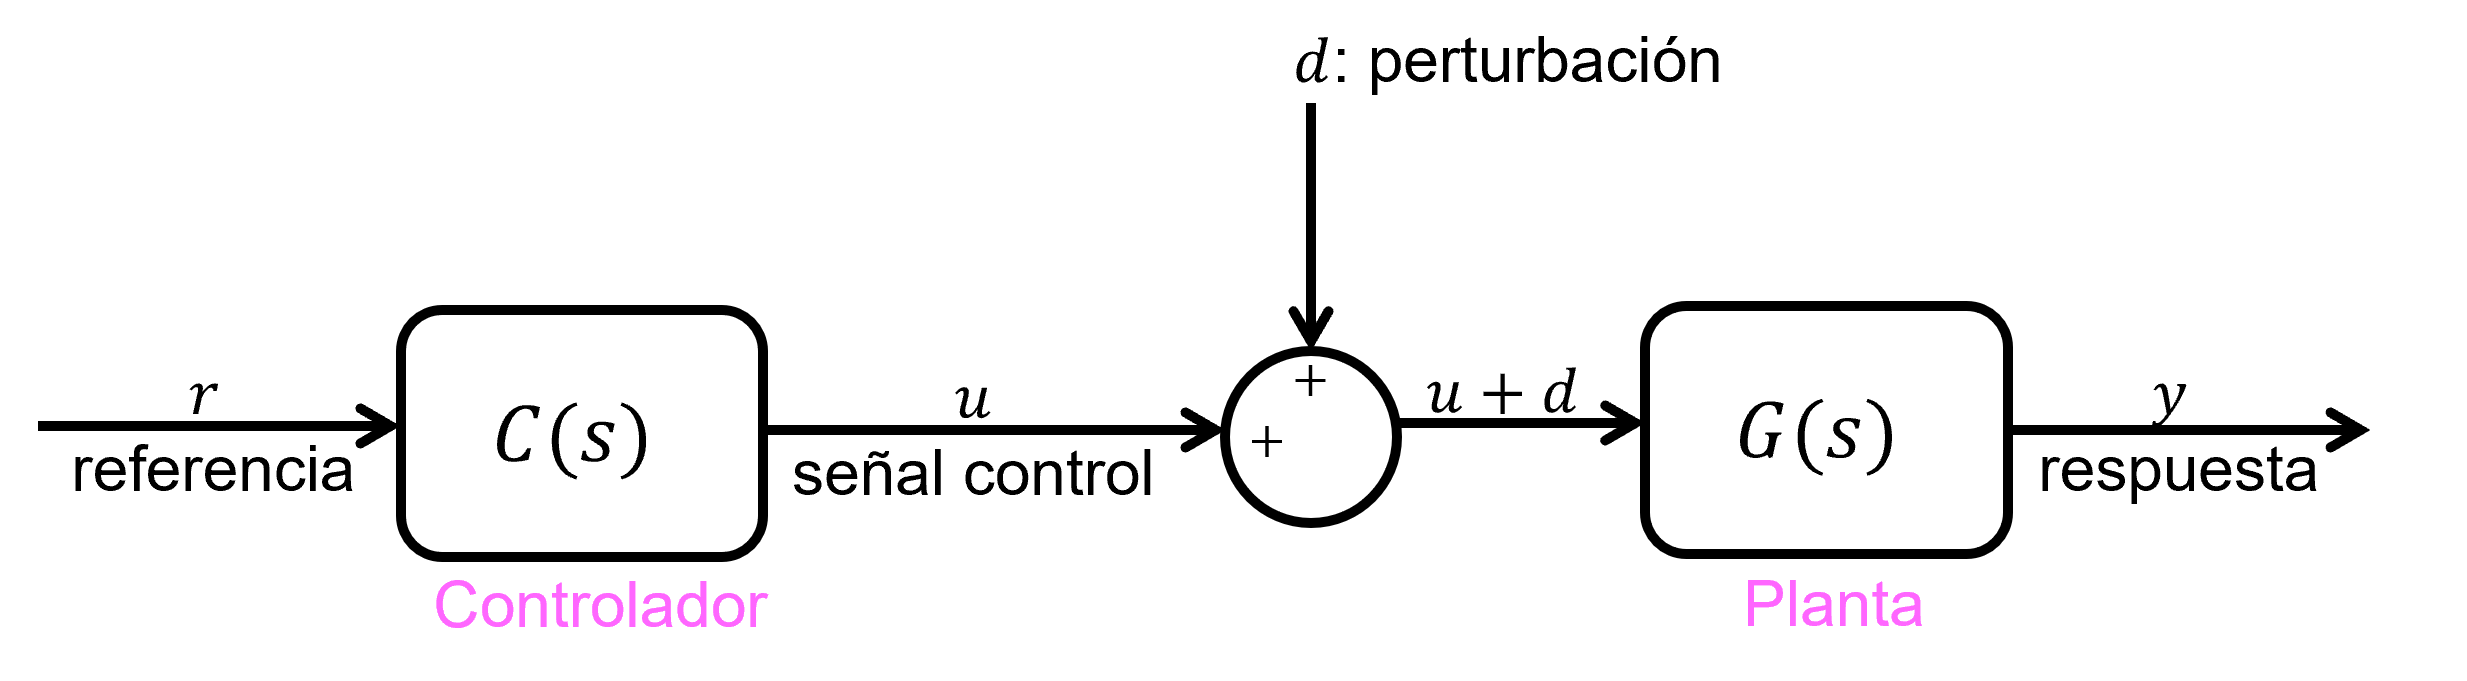
\includegraphics[scale=0.7]{Figuras/open-loop.png}
\end{figure}

\begin{itemize}
    \item[(1)] $Y(s)=G(s)[U(s)+D(s)]$, si asumimos $D(s)=0$
    \item[(2)] $U(s)=C(s)R(s)$
\end{itemize}

Reemplazar (2) en (1):
$$Y(s)=G(s)C(s)R(s)=L(s)R(s)$$
Donde $L(s)=G(s)C(s)$ es el sistema abierto ``open-loop system'' en representación función de transferencia.\\
\par Si buscamos: 
\begin{align*}
    y(t)&=r(t) ~/\mathcal{L}\{\cdot\}\\
    Y(s)&=R(s)\\
    \Longrightarrow L(s)&=1\\
    \Longrightarrow C(s)&=\frac{1}{G(s)} ~\text{``control inverso''}
\end{align*}

\underline{Nota}: 
\begin{itemize}
    \item Muy simple y ``barato'' (no hay necesidad de sensores)
    \item No es robusto $\Longrightarrow$ si hay incertidumbre en $G(s)$
    \begin{align*}
        L(s)&=G(s)C(s)\neq 1\\
        &=[\hat{G}(s)+\Delta(s)]\frac{1}{\hat{G}(s)}\\
        &=1+\frac{\Delta(s)}{\hat{G}(s)}
    \end{align*}
\end{itemize}
\underline{Nota}: podría ser útil en RTHS, porque la respuesta es instantánea.

\subsection{Closed-loop (feedback) control}
\begin{figure}[H]
\centering
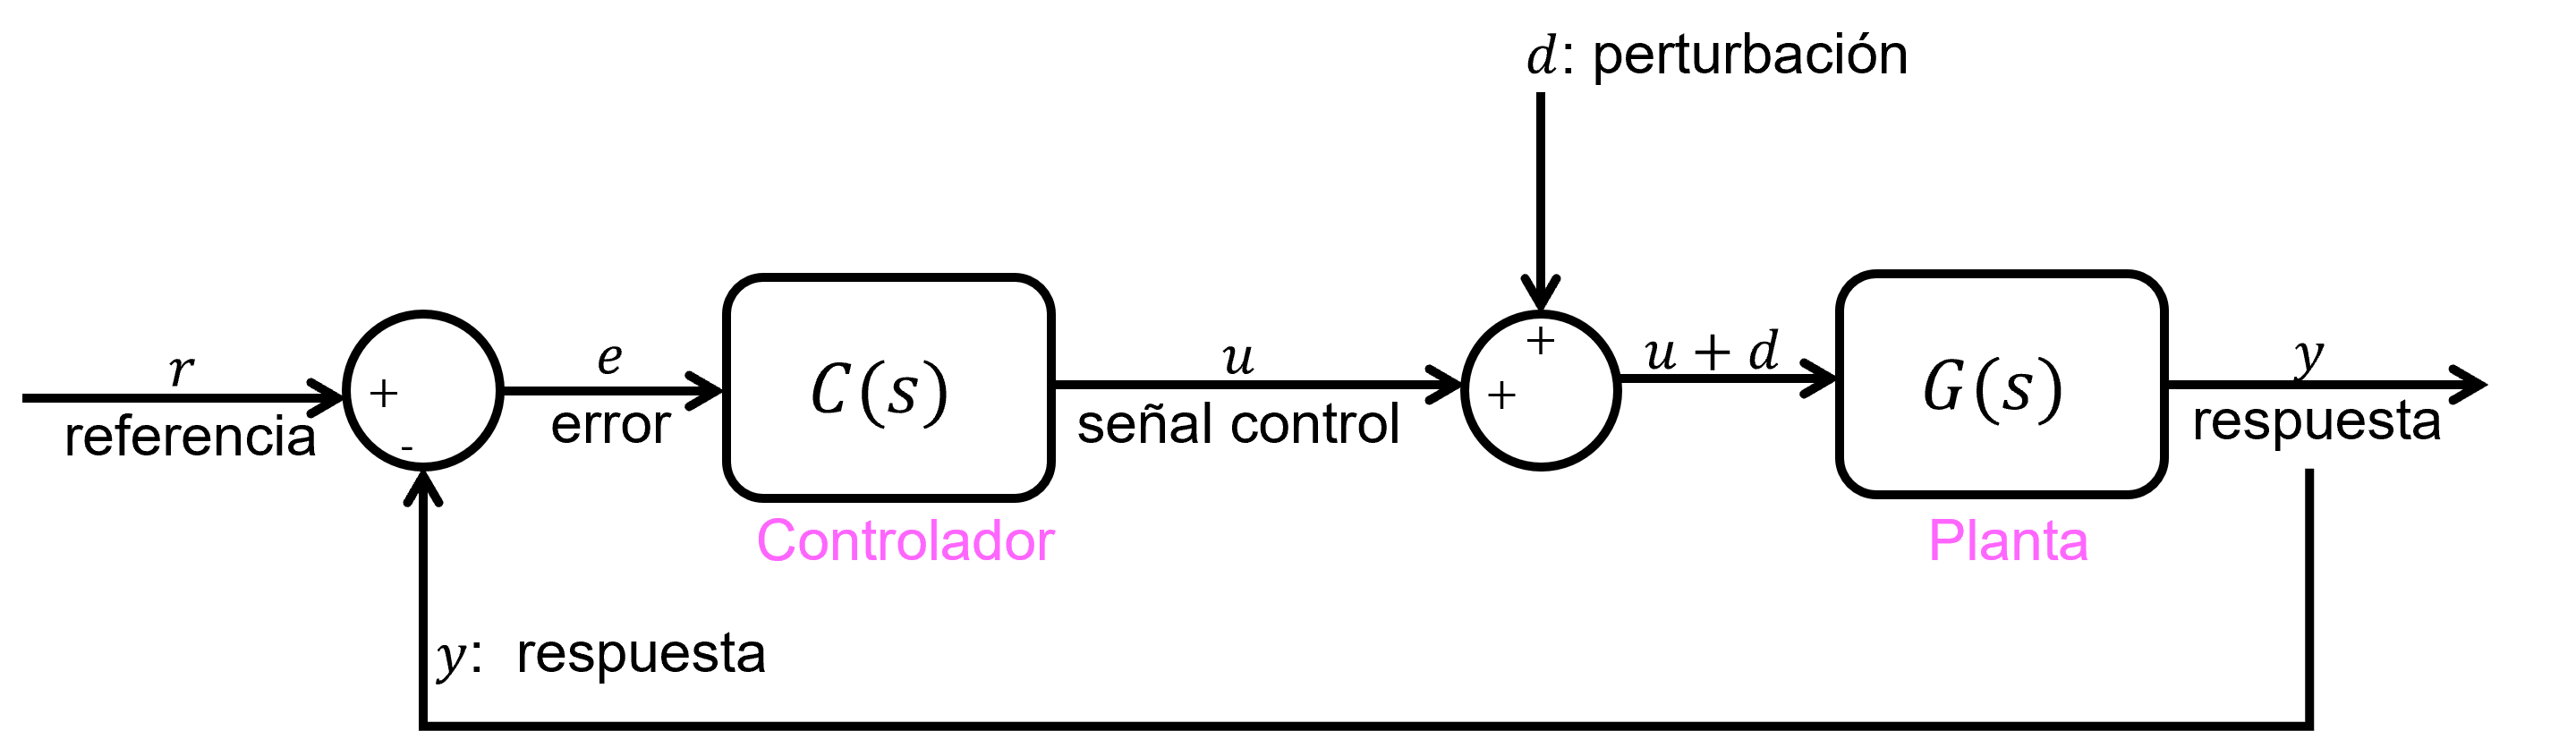
\includegraphics[scale=0.7]{Figuras/closed-loop.png}
\end{figure}

\begin{align*}
    \Longrightarrow & \text{Error: }~e(t)=r(t)-y(t)\\
    & \text{Si }e(t)=0\longrightarrow y(t)=r(t)
\end{align*}

\underline{Nota}:
\begin{itemize}
    \item Más robusto que feedforward $\Longrightarrow$ instalar sensores y ``alimentar'' la información de respuesta al controlador
    \item Más complicada y cara que open-loop
    \item Puede causar sistema estable o inestable
    \item Respuesta va a ser lenta $\Longrightarrow$ Real-time hybrid simulation
\end{itemize}

\subsubsection{Diagrama de Bloque}
Cuando se añade un dispositivo de control al sistema dinámico estructural, se genera un nuevo sistema dinámico con propiedades distintas.

\begin{figure}[H]
\centering
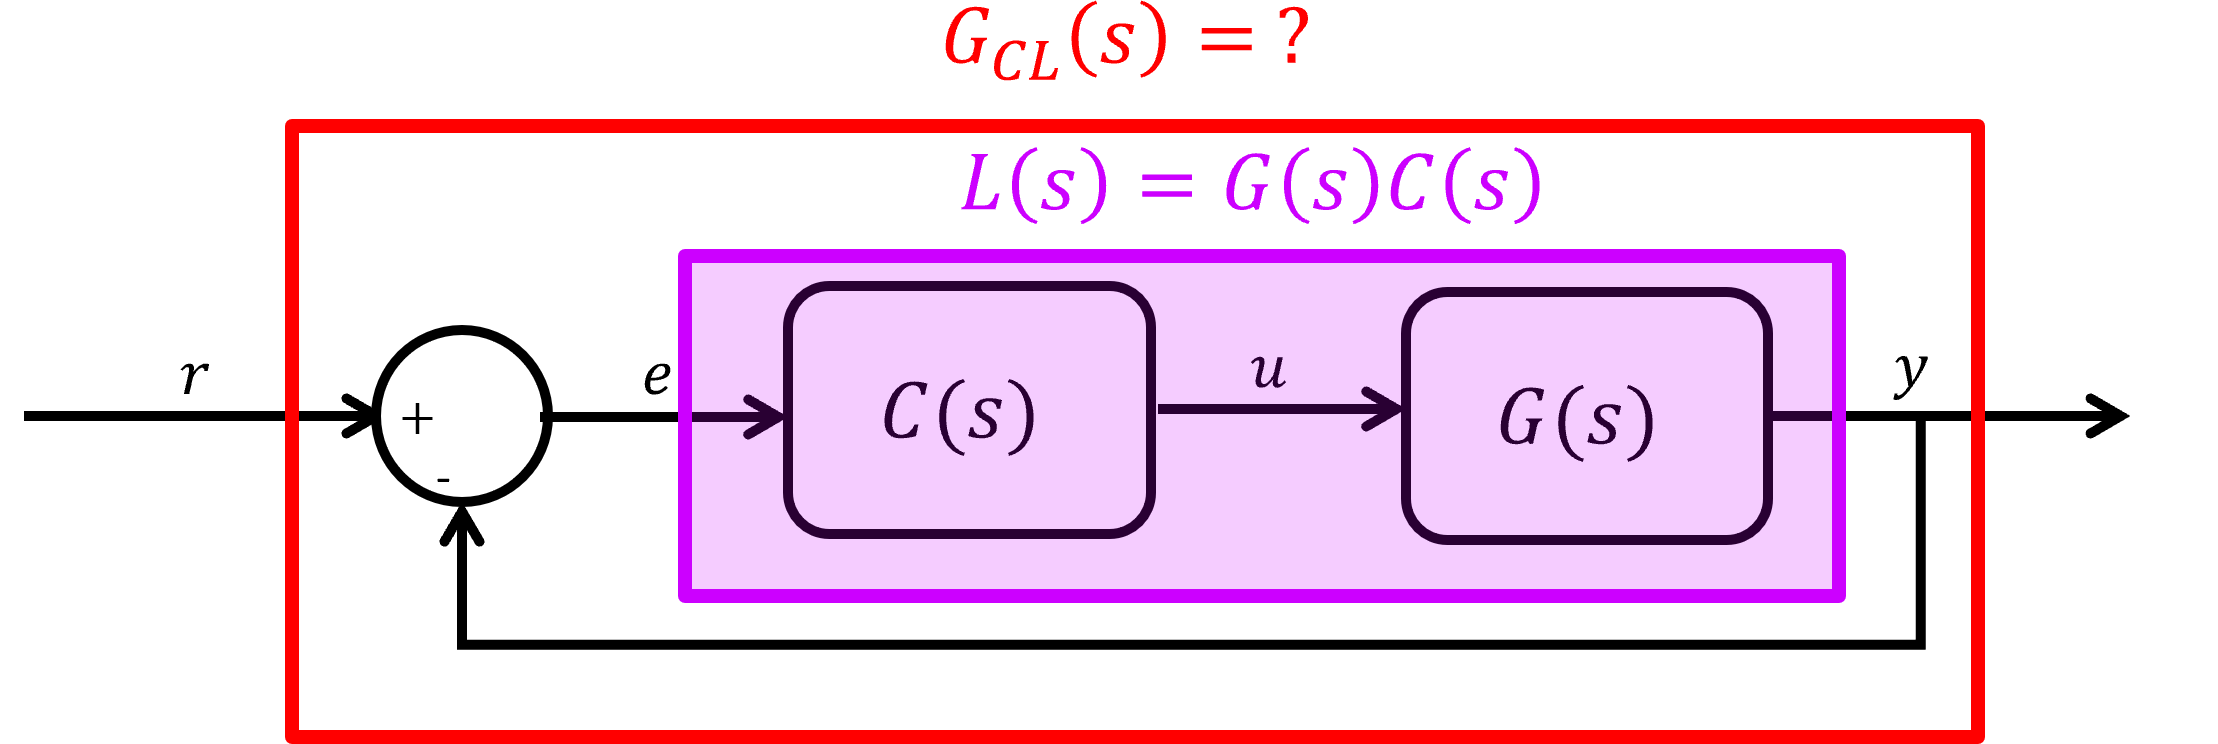
\includegraphics[scale=0.7]{Figuras/Diagrama_bloque.png}
\end{figure}

Desde el diagrama de bloques, se observa que:
\begin{align*}
    Y(s) = G(s)U(s)
\end{align*}

Pero, la señal de entrada $U(s)$ es la señal de salida del controlador:
\begin{align*}
    U(s) = C(s)E(s)
\end{align*}

Reemplazando, se obtiene que :
\begin{align*}
    Y(s) = G(s)C(s)E(s)
\end{align*}

Notar que la función de transferencia para este subsistema es $G(s)C(s)$. Siguiendo con el mísmo método reemplazando la señal de entrada por la multiplicación de su TF con su entrada (considerandola como salida):
\begin{align*}
    Y(s)&=L(s)E(s)=G(s)C(s)E(s)\\
    E(s)&=R(s)-Y(s)
\end{align*}

Reemplzando (2) en (1): 
\begin{align*}
    \Longrightarrow Y(s)&=G(s)C(s)[R(s)-Y(s)]\\
    \Longrightarrow[1+G(s)C(s)]Y(s)&=G(s)C(s)R(s)\\
    \Longrightarrow Y(s)&= \bigg[\frac{G(s)C(s)}{1+G(s)C(s)}\bigg]R(s)\\
    \Longrightarrow Y(s)&= G_{CL}(s)R(s)
\end{align*}

$\therefore G_{CL} = \bigg[\frac{G(s)C(s)}{1+G(s)C(s)}\bigg]$ es la función de transferencia del nuevo sistema que incorpora al controlador.

% \underline{Nota}: Vamos a ajustar $C(s)$ tal que $G_{CL}(s)$ tenga las propiedades deseadas en función de $t_r$, $M_p$ y $t_s$. O bien, elegir posición de los polos de $G_{CL}(s)$.

\section{Sistema estructural con Active Mass Damper (AMD)}
\begin{figure}[H]
\centering
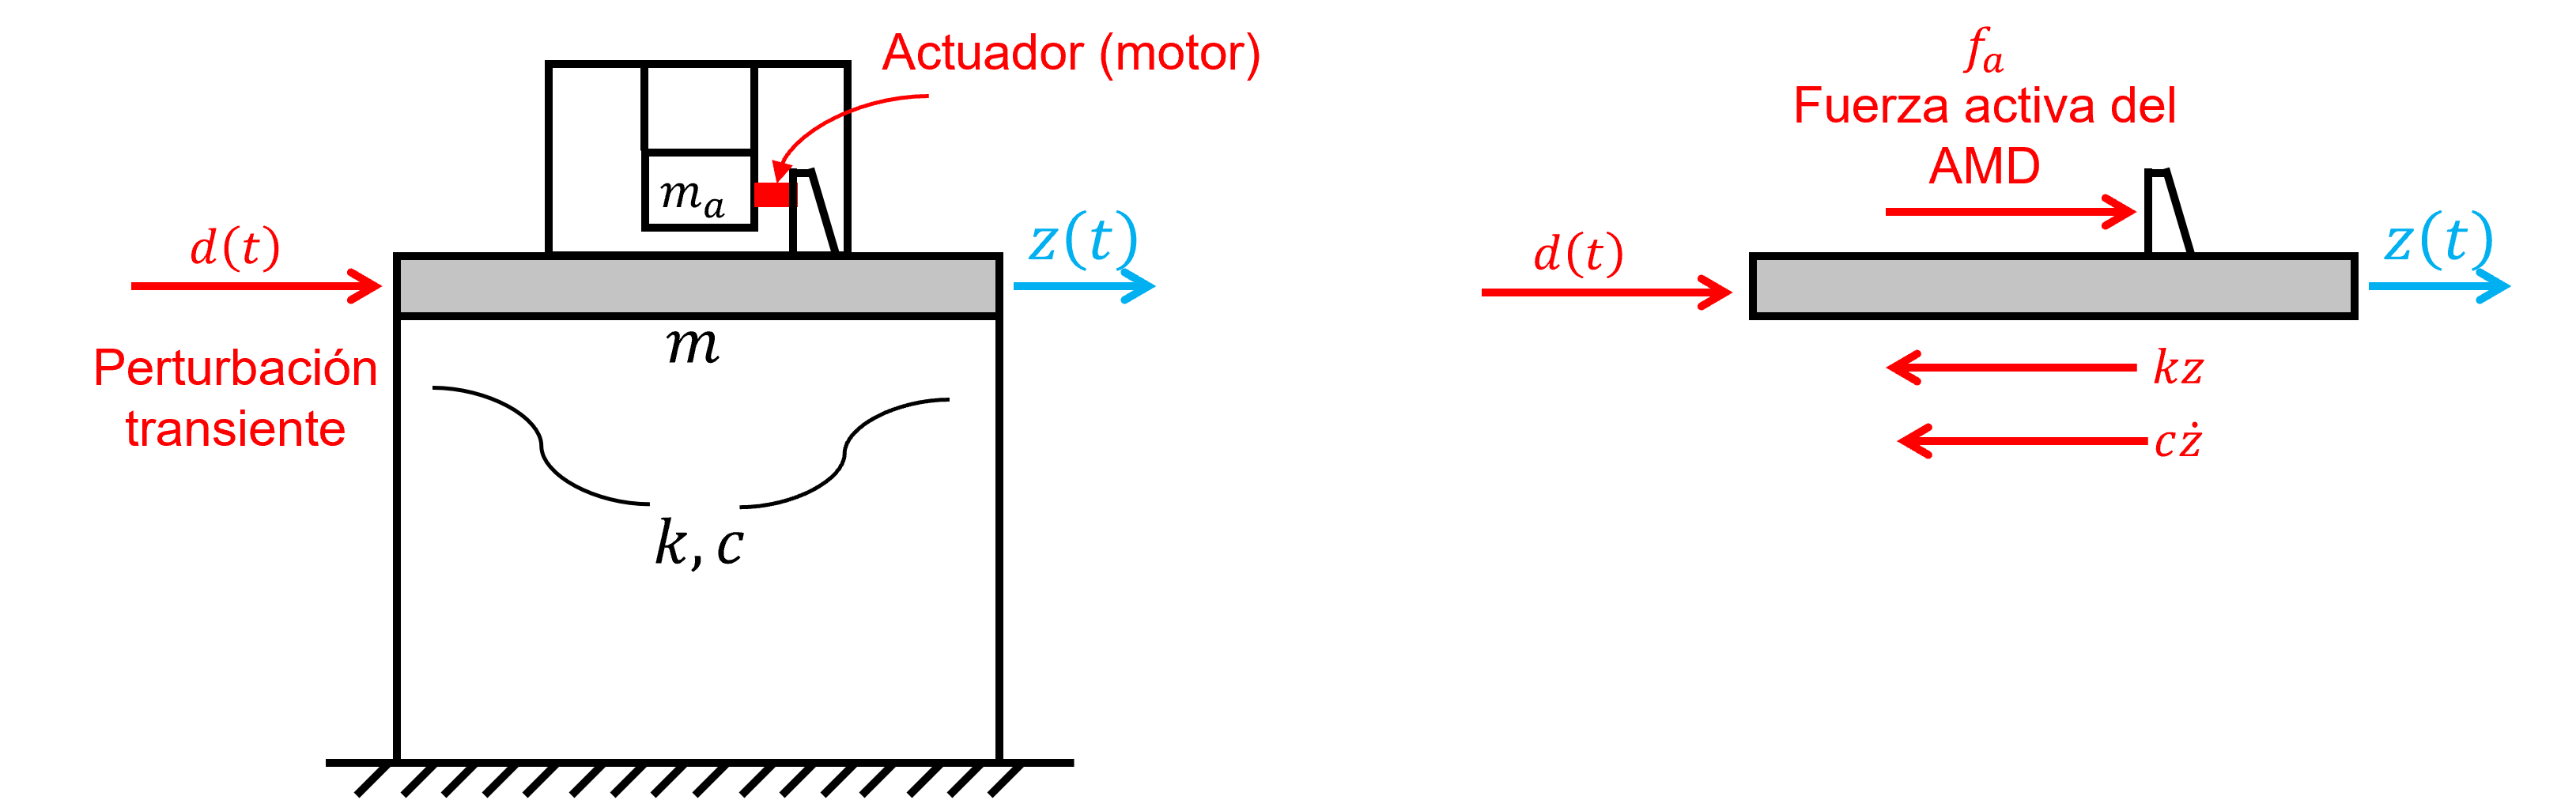
\includegraphics[scale=0.6]{Figuras/AMD.png}
\end{figure}
\begin{align*}
    \text{EDM: }~ m\ddot{z}+c\dot{z}+kz=f_a(u)+\cancelto{\text{Asuma=0}}{d}
\end{align*}
$u$: señal control (voltaje)\\
El objetivo es diseñar un \underline{algoritmo de control} $f_a(u,t)$ para mitigar $z(t)$ y mejorar el desempeño.


% \section{Respuesta transiente}
% Si queremos transicionar de un estado $x(t_0)$ a $x_2$, la respuesta no es instantánea y existe una respuesta transiente que hay que limitar.
% \begin{figure}[H]
% \centering
% 
\includegraphics[scale=0.6]{step.png}
% \end{figure}
% \underline{Definición}:
% \begin{itemize}
%     \item \underline{Tiempo de subida} (``rise time'', $t_r$): tiempo que toma subir. Ej.: ir desde 10\% hasta 90\% de respuesta o de 0\% a 100\%.
%     \item \underline{Sobreimpulso} (``overshoot'', $M_p$): exceso de respuesta transitoria sobre la referencia deseada.
%     \item \underline{Tiempo de asentamiento} (``senttling time'', $t_s$): tiempo que toma el sistema en decaer hasta 1\%
% \end{itemize}

\section{Teorema del Límite Final}
\begin{figure}[H]
\centering
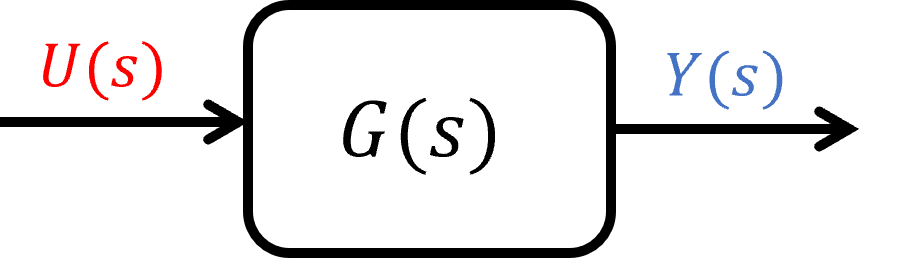
\includegraphics[scale=0.7]{Figuras/planta2.png}
\end{figure}
Respuesta Estado Estacionario: $y_\infty=\lim_{t\to\infty} y(t)$\\
\par Válido si y solo si $G(s)$ es estable.\\
\par \underline{Teorema}: Si todos los polos de $G(s)$ se encuentran a la izquierda del plano complejo, entonces:
\begin{align*}
    \lim_{t\to\infty} y(t)=\lim_{s\to 0} sY(s)
\end{align*}


\section{Requisitos de control}
\begin{figure}[H]
\centering
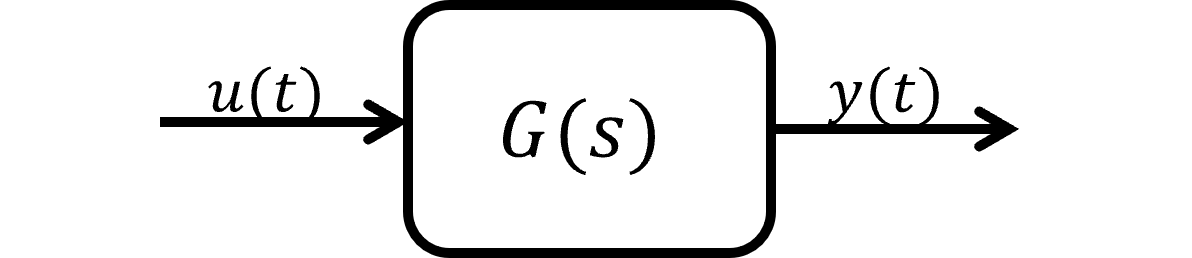
\includegraphics[scale=0.7]{Figuras/Planta.png}
\end{figure}
$\Longrightarrow$ Generar un set de requisitos de respuesta de planta $\Longrightarrow$ Especificaciones de respuesta transiente ante un escalón unitario
\begin{itemize}
    \item $t_r$ (tiempo de subida)
    \item $M_p$ (sobreimpulso)
    \item $t_s$ (tiempo de asentamiento)
\end{itemize}

\subsection{Especificaciones de Respuesta Transiente}

Ref: \textcite[Sec. 3.4]{Franklin2015}

Suponiendo un sistema LTI-SISO de segundo orden:\\

\begin{align*}
    \text{EDM: }~ m\ddot{u}+c\dot{u}+ku &= f\\
    \Longrightarrow H_{UF}(s) &= \frac{1/m}{s^2+2\zeta\omega_n s+\omega_n^2}
\end{align*}

Polos del sistema:

\begin{align*}
    s_{1,2} &= -\underbrace{\zeta \omega_n}_{\sigma} \pm j \underbrace{\omega_n \sqrt{1 - \zeta^2}}_{\omega_d} \\
    &= - \sigma \pm j \omega_d
\end{align*}

\begin{figure}[H]
    \centering
    
\includegraphics[scale=0.5]{transiente.png}
\end{figure}



Fórmulas para estimar la respuesta transiente para el caso de excitación escalón:

% Nota: Estas formulas son distintas a las descritas en la literatura para $\zeta = 50\%$, ver libro Franklin "Feedback Control"

\begin{itemize}
    \item \underline{Tiempo subida, $t_r$}: Asumiento $\zeta=2\%$, 
    $$t_r\approx \frac{1.6}{\omega_n}$$
    \item \underline{Sobreimpulso, $M_p$}: 
    $$-\log \left(\frac{M_p}{\pi} \right) \approx \tan(\theta)$$
    \item \underline{Tiempo asentamiento, $t_s$}: Asumiendo 2\% de respuesta esperada en ``steady-state'',
    $$t_s\approx \frac{4}{\zeta \omega_n} $$
\end{itemize}

\subsection{``Pole placement'', ubicación de polos}
Dadas las especificaciones transientes: $t_r$, $M_p$, $t_s$
\begin{align*}
    \color{VioletRed}{t_s}&<(t_s)_{lim}=\frac{4}{(\zeta\omega_n)_{lim}}\\
    \color{BurntOrange}{t_r}&<(t_r)_{lim}\approx \frac{1.6}{\omega_n}\\
    \color{LimeGreen}{M_p}&<(M_p)_{lim}=e^{-\pi\tan(\theta)}
\end{align*}

\begin{figure}[H]
\centering

\includegraphics[scale=0.7]{pole_placement.png}
\end{figure}


\section{Control PID}
El control PID es un \underline{algoritmo de control} para diseñar la señal de control $u(t)$ para definir nuestra fuerza de control $f_a(u,t)$ es el control PID.
\begin{align*}
    u(t)&=K_pe(t)+K_D\frac{de(t)}{dt}+K_I\int e(t)dt\\
    \Longleftrightarrow U(s) &= K_pE(s)+K_DsE(s)+K_I\frac{E(s)}{s} \\
    \Longleftrightarrow U(s) &= \left(K_P + K_Ds + \frac{K_I}{s}\right)E(s)
\end{align*}

Si definimos $C(s) = K_P + K_Ds + \frac{K_I}{s}$
\begin{align*}
    U(s) = C(s)E(s)
\end{align*}
\begin{itemize}
    \item $K_p$: control proporcional
    \item $K_D$: control derivativo
    \item $K_I$: control integral
    \item $K_p e(t)$: error instantáneo
    \item $K_D \frac{de(t)}{dt}$: error futuro
    \item $K_I \int e(t) dt$: error pasado
    \item $e(t) = r(t) - y(t)$
\end{itemize}

\begin{figure}[H]
\centering
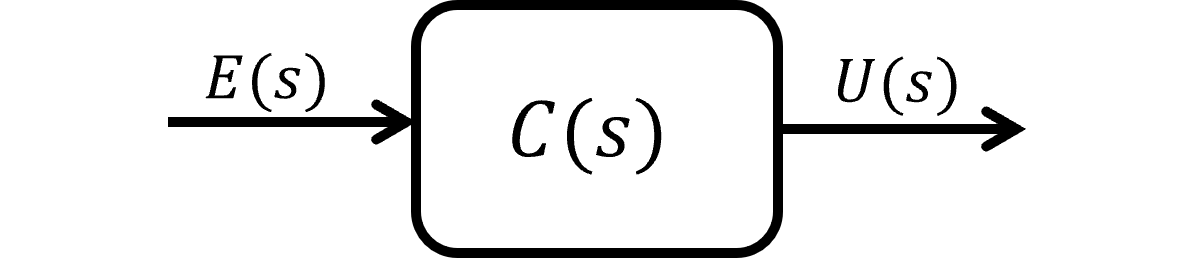
\includegraphics[scale=0.7]{Figuras/controlador.png}
\end{figure}

\begin{figure}[H]
\centering
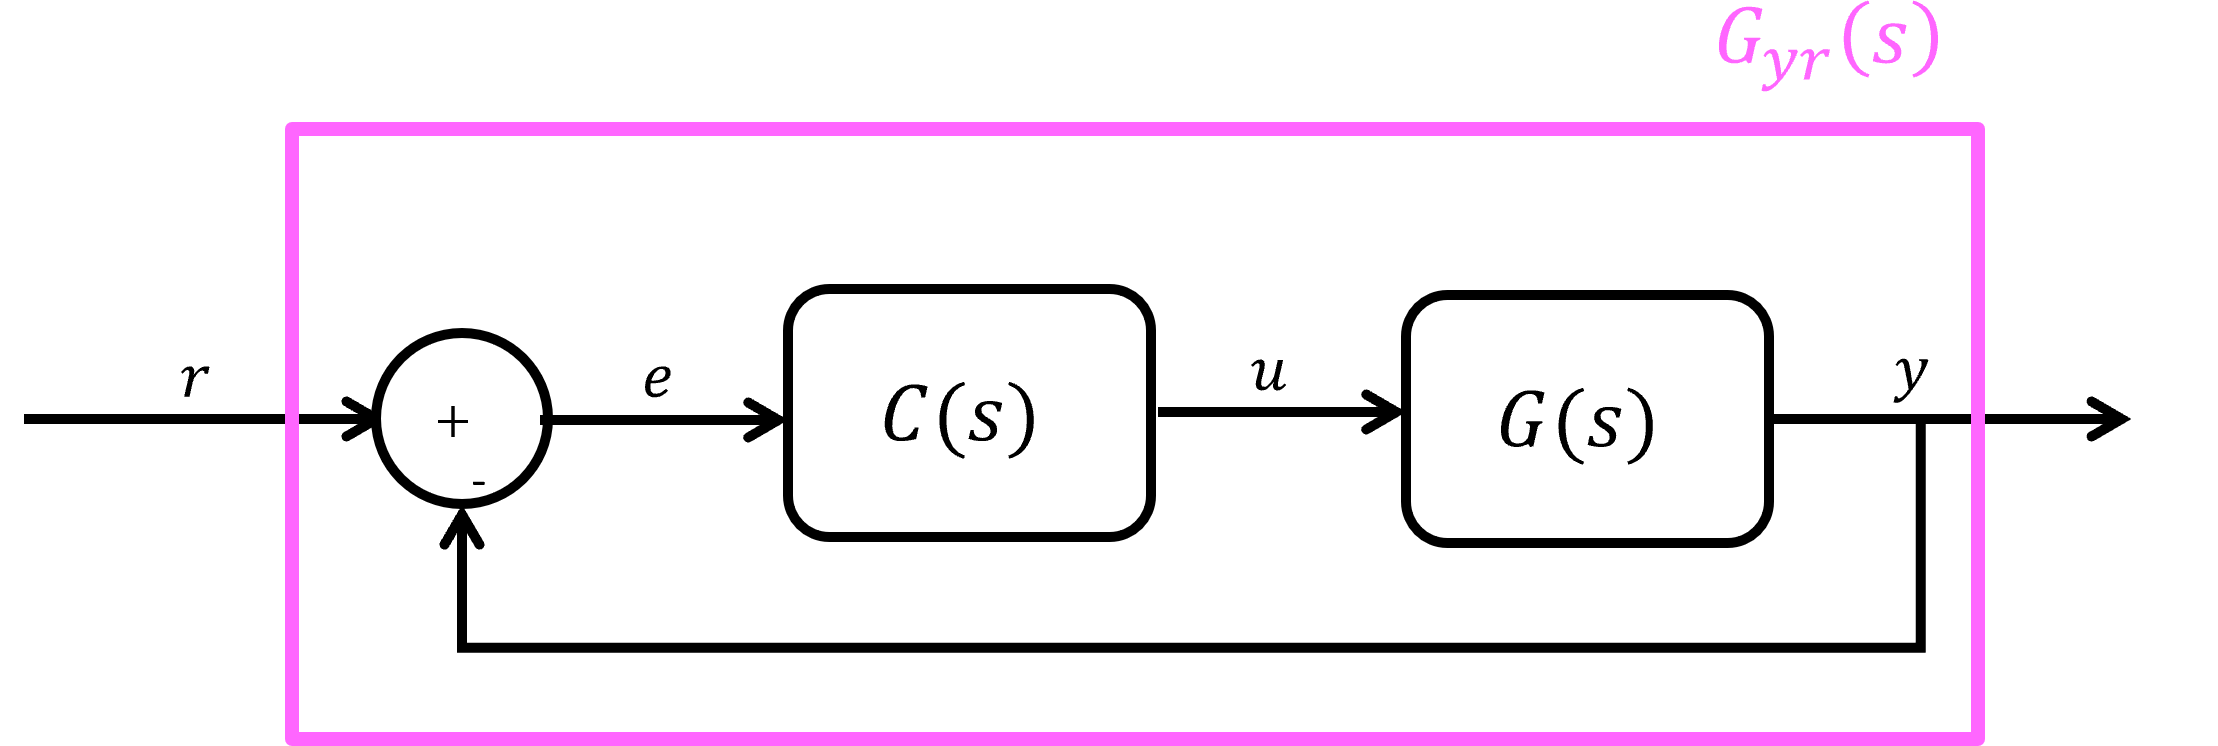
\includegraphics[scale=0.7]{Figuras/PID2.png}
\end{figure}
$C(s)$ se diseña tal que $e(t)\to 0$
$$C(s)=K_p+\frac{K_I}{s}+K_Ds$$
\begin{itemize}
    \item $Y(s)=G(s)U(s)$
    \item $U(s)=C(s)E(S)$
    \item $E(s)=R(s)-Y(s)$
\end{itemize}
\begin{align*}
    Y(s)&=G(s)C(s)[R(s)-Y(s)]\\
    \Longrightarrow Y(s)&=\frac{G(s)C(s)}{1+G(s)C(s)}R(s)\\
    &=G_{CL}R(s)\\
    &=G_{yr}R(s)
\end{align*}

\subsection{Control P}
Si se considera únicamente el control P (proporcional), se puede obtener la función de transferencia del sistema cerrado.
\begin{align*}
    & C(s)=K_p\\
    \Longrightarrow & G(s)=\frac{1}{ms^2+cs+k}=\frac{1/m}{s^2+2\zeta\omega_n s+\omega_n^2}=\frac{c}{s^2+as+b}\\
    \Longrightarrow & G_{CL}(s)=\frac{K_p\frac{c}{s^2+bs+c}}{1+K_p\frac{c}{s^2+bs+c}} \\
    \Longrightarrow & G_{CL}(s)=\frac{K_p c}{s^2+as+(b+K_p\cdot c)} \longrightarrow \text{Función de transferencia Closed-loop}
\end{align*}

Al tener la misma forma de un sistema 1GDL, se pueden definir propiedades equivalentes:
\begin{align*}
    \Longrightarrow & \omega_{n,CL}= \sqrt{b+K_p\cdot c}\\
    \Longrightarrow & \zeta_{CL}= \frac{a}{2\omega_{n,CL}}=\frac{a}{2\sqrt{b+K_p\cdot c}}
\end{align*}

Notar que:
\begin{itemize}
    \item Aumentar $K_p$ hace que $\omega_{n,CL}$ aumente (sistema rígido)
    \item Aumentar $K_p$ hace que $\zeta$ disminuya
\end{itemize}

En términos de la respuesta $y_{\infty}$: 
\begin{align*}
    y_{\infty}=\lim_{s\to 0}sY_{CL}(s)=\lim_{s\to 0} sG_{CL}(s)R(s)
\end{align*}
Con $R(s)$: escalón unitario

\begin{align*}
    \Longrightarrow y_{\infty}=\lim_{s\to 0} s\frac{K_p\cdot c}{s^2+as+(b+K_p\cdot c)}\cdot\frac{1}{s}=\frac{K_p\cdot c}{b+K_p \cdot c}\neq 1
\end{align*}
Valores pequeños de $K_p\Longrightarrow$ error en estado estacionario
\begin{figure}[H]
\centering
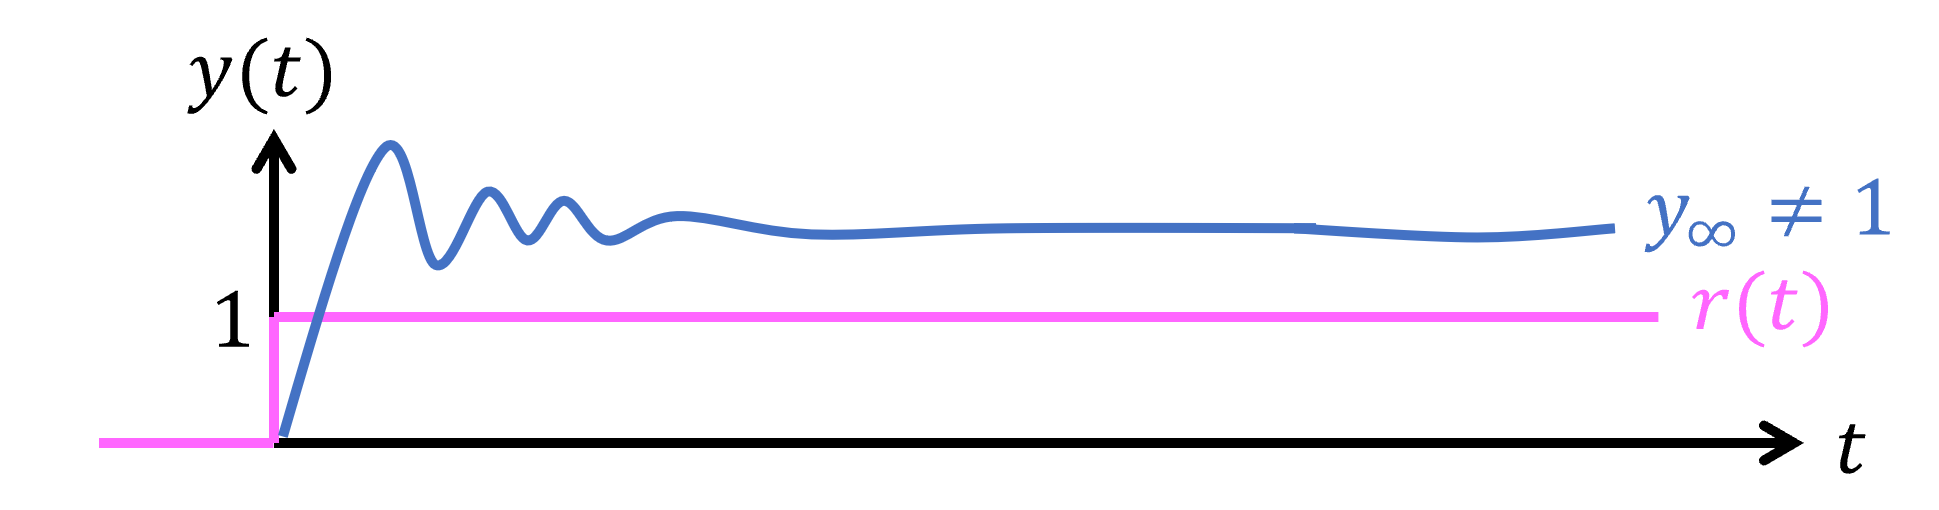
\includegraphics[scale=0.7]{Figuras/controlP.png}
\end{figure}

\subsection{Control PD}
Análogamente al control P, se puede obtener la función de transferencia de un sistema estructural con control PD
\begin{align*}
    G_{CL}(s)&=\frac{G(s)C(s)}{1+G(s)C(s)}=\frac{\left(\frac{c}{s^2+as+b}\right)C(s)}{1+\left(\frac{c}{s^2+as+b}\right)C(s)}\\
    & = \frac{c\cdot C(s)}{a^2+as+\left( b+c \cdot C(s) \right)}
\end{align*}

Si el controlador es PD, entonces se obtiene la expresión para el sistema cerrado:
\begin{align*}
    C(s) &= K_p+K_Ds=K_p(1+T_Ds)\\
    \Longrightarrow G_{CL} &= \frac{cK_p(1+T_Ds)}{s^2+(a+cbK_pT_D)s+b(1+K_p)}
\end{align*}

\begin{itemize}
    \item Aparece un ``cero'' en el numerador
    \item Podemos controlar $\omega_{n,CL}$ mediante $K_p$
    \item Podemos controlar $\zeta_{CL}$ mediante una combinación de $K_p$ y $T_D$
\end{itemize}

$\Longrightarrow y_{\infty}$, no hay cambio en el error de estado estacionario\\
\par $\Longrightarrow$ Con PD podemos ubicar los polos del sistema cerrado donde nosotros queramos\\
\par \underline{Advertencia}: Control D amplifica el ruido eléctrico en la señal de respuesta $\Longrightarrow$ Nunca utilizar control D.

\subsection{Control PI}
\begin{align*}
    \Longrightarrow G_{CL}(s) &= \frac{c\cdot C(s)}{s^2+as+\left(b+c \cdot C(s)\right)}\\
    \Longrightarrow C(s) &= K_p +\frac{K_I}{s}=K_P\left(1+\frac{T_I}{2}\right)\\
    \Longrightarrow G_{CL} &= \frac{cK_p(s+T_I)}{s^3+as^2+(b+cK_p)s+cK_pT_I}
\end{align*}

\begin{align*}
    \Longrightarrow y_{\infty}=\lim_{s\to 0}sY_{CL}(s)=\lim_{s\to 0} s\frac{K_p\cdot c(s+T_I)}{s^3+as^2+(b+cK_p)s+cK_pT_I}\cdot\frac{1}{s}=\frac{T_IK_p\cdot c}{T_IK_p\cdot c}= 1
\end{align*}

\underline{Nota}: El esfuerzo del control I genera una reducción del error en estado estacionario.

\subsection{Control PID}
\begin{align*}
    C(s) &= K_p+\frac{K_I}{s}+K_Ds\\
    &= K_p\left(1+\frac{T_I}{s}+T_Ds\right)
\end{align*}

\begin{itemize}
    \item Aumentar $K_p$: Sistema que responde rápido, pero se genera alto sobreimpulso, y el error estacionario alto.
    \item Aumentar $K_D$: Agregar amortiguameinto al sistema (disminuir sobreimpulso), pero puede amplificar el ruido eléctrico.
    \item Aumentar $K_I$: Reducir el error en estado estacionario, sistema se vuelve más lento.
\end{itemize}

\begin{table}[H]
    \centering
    \begin{tabular}{c|c|c|c|}
                & $K_p \uparrow$ & $K_D \uparrow$ & $K_I \uparrow$\\ \hline
         error ss & $\downarrow$ & - & 0\\ \hline
         $t_r$ & $\downarrow$ & - & ? \\ \hline
         $t_s$ & - & $\downarrow$ & ? ($\uparrow$)\\ \hline
         $M_p$ & $\uparrow$ & $\downarrow$ & ? ($\uparrow$)\\ 
    \end{tabular}
\end{table}



\section{Ejemplo: Simulación control PID mediante Simulink}
\begin{figure}[H]
\centering
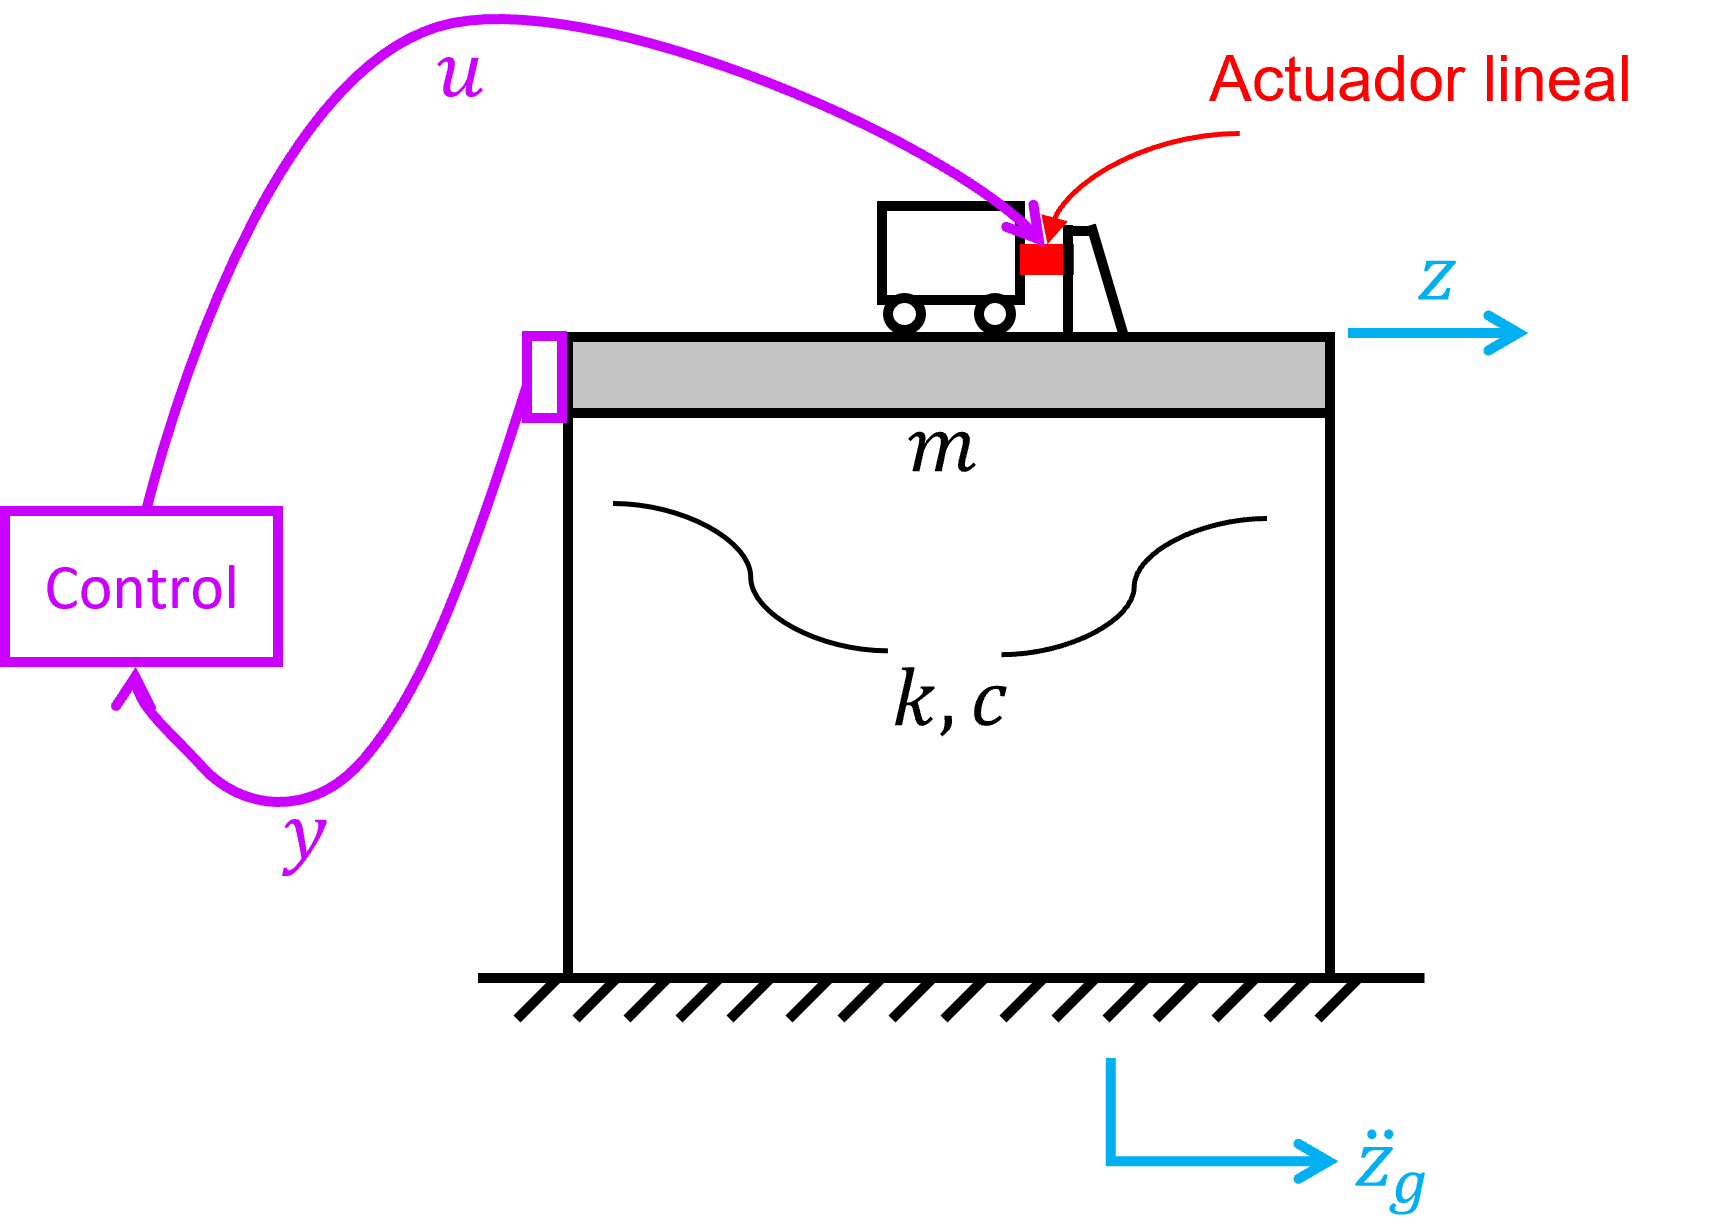
\includegraphics[scale=0.7]{Figuras/simulink_modelo.png}
\end{figure}

\begin{align*}
    \text{EDM: }~ m\ddot{z}+c\dot{z}+kz=-m\ddot{z}_g+gu
\end{align*}

\underline{Propiedades de la estructura}: 
\begin{itemize}
    \item $m=100$ Kg
    \item $c=50$ Ns/m
    \item $k=4000$ N/m
    \item $g=100$ N/V
\end{itemize}

\underline{Representación espacio-estado}: 
\begin{align*}
    {x}=\begin{bmatrix}{z}\\ {\dot{z}}\end{bmatrix}, \quad u_1 =\ddot{z}_g, \quad u_2=u
\end{align*}

\begin{align*}
    {\dot{x}} &=
    \begin{bmatrix}
    0 & 1\\
    -k/m & -c/m
    \end{bmatrix}{x} +
    \begin{bmatrix}
    0 \\ -1
    \end{bmatrix}u_1+
    \begin{bmatrix}
    0 \\ g/m
    \end{bmatrix}u_2 \\
    &= \begin{bmatrix} 0 & 1\\-k/m & -c/m
    \end{bmatrix}{x} +
    \begin{bmatrix}
    0 & 0\\ -1 & g/m
    \end{bmatrix} 
    \begin{bmatrix}
    \ddot{z}_g\\ u
    \end{bmatrix}
\end{align*}

\begin{align*}
    {y}&=[z]\\
    {y}&= \begin{bmatrix}1 & 0 \end{bmatrix}{x}+\begin{bmatrix}0 & 0 \end{bmatrix}\begin{bmatrix}
    \ddot{z}_g\\ u
    \end{bmatrix}
\end{align*}

\begin{align}
    {u}=\begin{bmatrix}
    \ddot{z}_g\\ u
    \end{bmatrix}\longrightarrow
    \begin{array} {|r|r|}
      \hline A & B \\
      \hline C & D \\
      \hline 
    \end{array}
    \longrightarrow {y}=[z] \quad \text{Sistema ``MISO''}
\end{align}


\underline{Objetivo}: Diseñar un control PID para mejorar el desempeño de la estructura sometida al terremoto de Northridge 1994.\\
\par \underline{Contol PID}: 
\begin{align*}
    C(s)&=K_p\bigg(1+\frac{T_I}{s}+T_Ds\bigg)\\
    &= K_p+\frac{K_I}{s}+K_Ds, \quad K_I=K_pT_I, \quad K_D=K_pT_D
\end{align*}

% \begin{multicols}{2}
% \underline{Código Matlab}: 
% \begin{minted}[]{matlab}
% %% Simulacion Control PID
% % Gaston Fermandois, 2020

% %% Inicializar
% clear all, close all, clc

% %% Parametros

% m=100; % masa primer piso, kg
% c=50; %Ns/m
% k=4000; %N/m
% g=100; %cte motor, N/V

% %% Control PID

% Kp=1;
% Ti=1/10; Ki=Kp*Ti;
% Td=1/100; Kd=Kp*Td;

% s=tf('s');
% Cpid=Kp*(1+Ti/s+Td*s);

% %% Espacio estado

% A=[0 1;-k/m -c/m];
% B1=[0;-1];
% B2=[0;g/m];
% B=[B1 B2];
% C=[1 0];
% D1=0;
% D2=0;
% D=[D1 D2];

% sys=ss(A,B,C,D);

% sysyu=ss(A,B2,C,D2);

% Gyu=tf(sysyu);

% %% Sistema Cerrado

% Gcl=Gyu*Cpid/(1+Gyu*Cpid);
% Gcl=minreal(Gcl) % Cancelación polos y ceros

% figure;
% rlocus(Gcl)

% %% Simulacion

% Tfinal=60; %s
% Fs=1000; %Hz
% Ts=1/Fs; %s

% GM=importdata('RegistroNorthridge1994.txt');
% N=length(GM.data);
% dt=0.02; %s
% t=linspace(0,N*dt,N);
% ddzg=[t.' GM.data/100]; %[s m/s2]

% sim('AMDctrl_demo_simu')
% \end{minted}
% \end{multicols}

\underline{Código Matlab}: 

\begin{lstlisting}[style=matlab-editor]
%% Parametros
m=100; % masa primer piso, kg
c=50; %Ns/m
k=4000; %N/m
g=100; %cte motor, N/V

%% Control PID
Kp=1;
Ti=1/10; Ki=Kp*Ti;
Td=1/100; Kd=Kp*Td;
s=tf('s');
Cpid=Kp*(1+Ti/s+Td*s);

%% Espacio estado
A=[0 1;-k/m -c/m];
B1=[0;-1];
B2=[0;g/m];
B=[B1 B2];
C=[1 0];
D1=0;
D2=0;
D=[D1 D2];
sys=ss(A,B,C,D);
sysyu=ss(A,B2,C,D2);
Gyu=tf(sysyu);

%% Sistema Cerrado
Gcl=Gyu*Cpid/(1+Gyu*Cpid);
Gcl=minreal(Gcl) % Cancelacion polos y ceros

figure;
rlocus(Gcl)

%% Simulacion
Tfinal=60; %s
Fs=1000; %Hz
Ts=1/Fs; %s

GM=importdata('RegistroNorthridge1994.txt');
N=length(GM.data);
dt=0.02; %s
t=linspace(0,N*dt,N);
ddzg=[t.' GM.data/100]; %[s m/s2]

sim('AMDctrl_demo_simu')
\end{lstlisting}


\underline{Simulink}:

\begin{figure}[H]
\centering
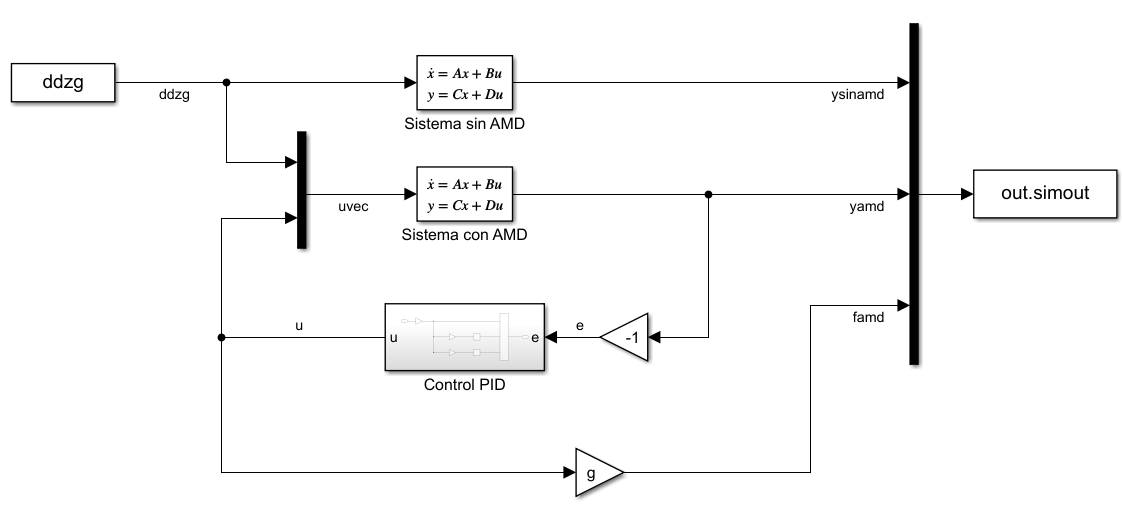
\includegraphics[scale=0.7]{Figuras/Simulink.png}
\end{figure}

\section{Root Locus}
$\Longrightarrow$ ``Migración de polos'', Locus = posición en latín
\begin{align*}
    \text{Planta: }~ G_{y\ddot{z}_g}(s)&=\frac{1/m}{s^2+2\zeta\omega_n s+\omega_n^2}\\
    G_{yu}(s) &=\frac{g/m}{s^2+2\zeta\omega_n s+\omega_n^2}
\end{align*}
\begin{align*}
    \text{Controlador PID: }~C(s)=K_p(1+\frac{T_I}{s}+T_Ds)
\end{align*}

\begin{figure}[H]
\centering
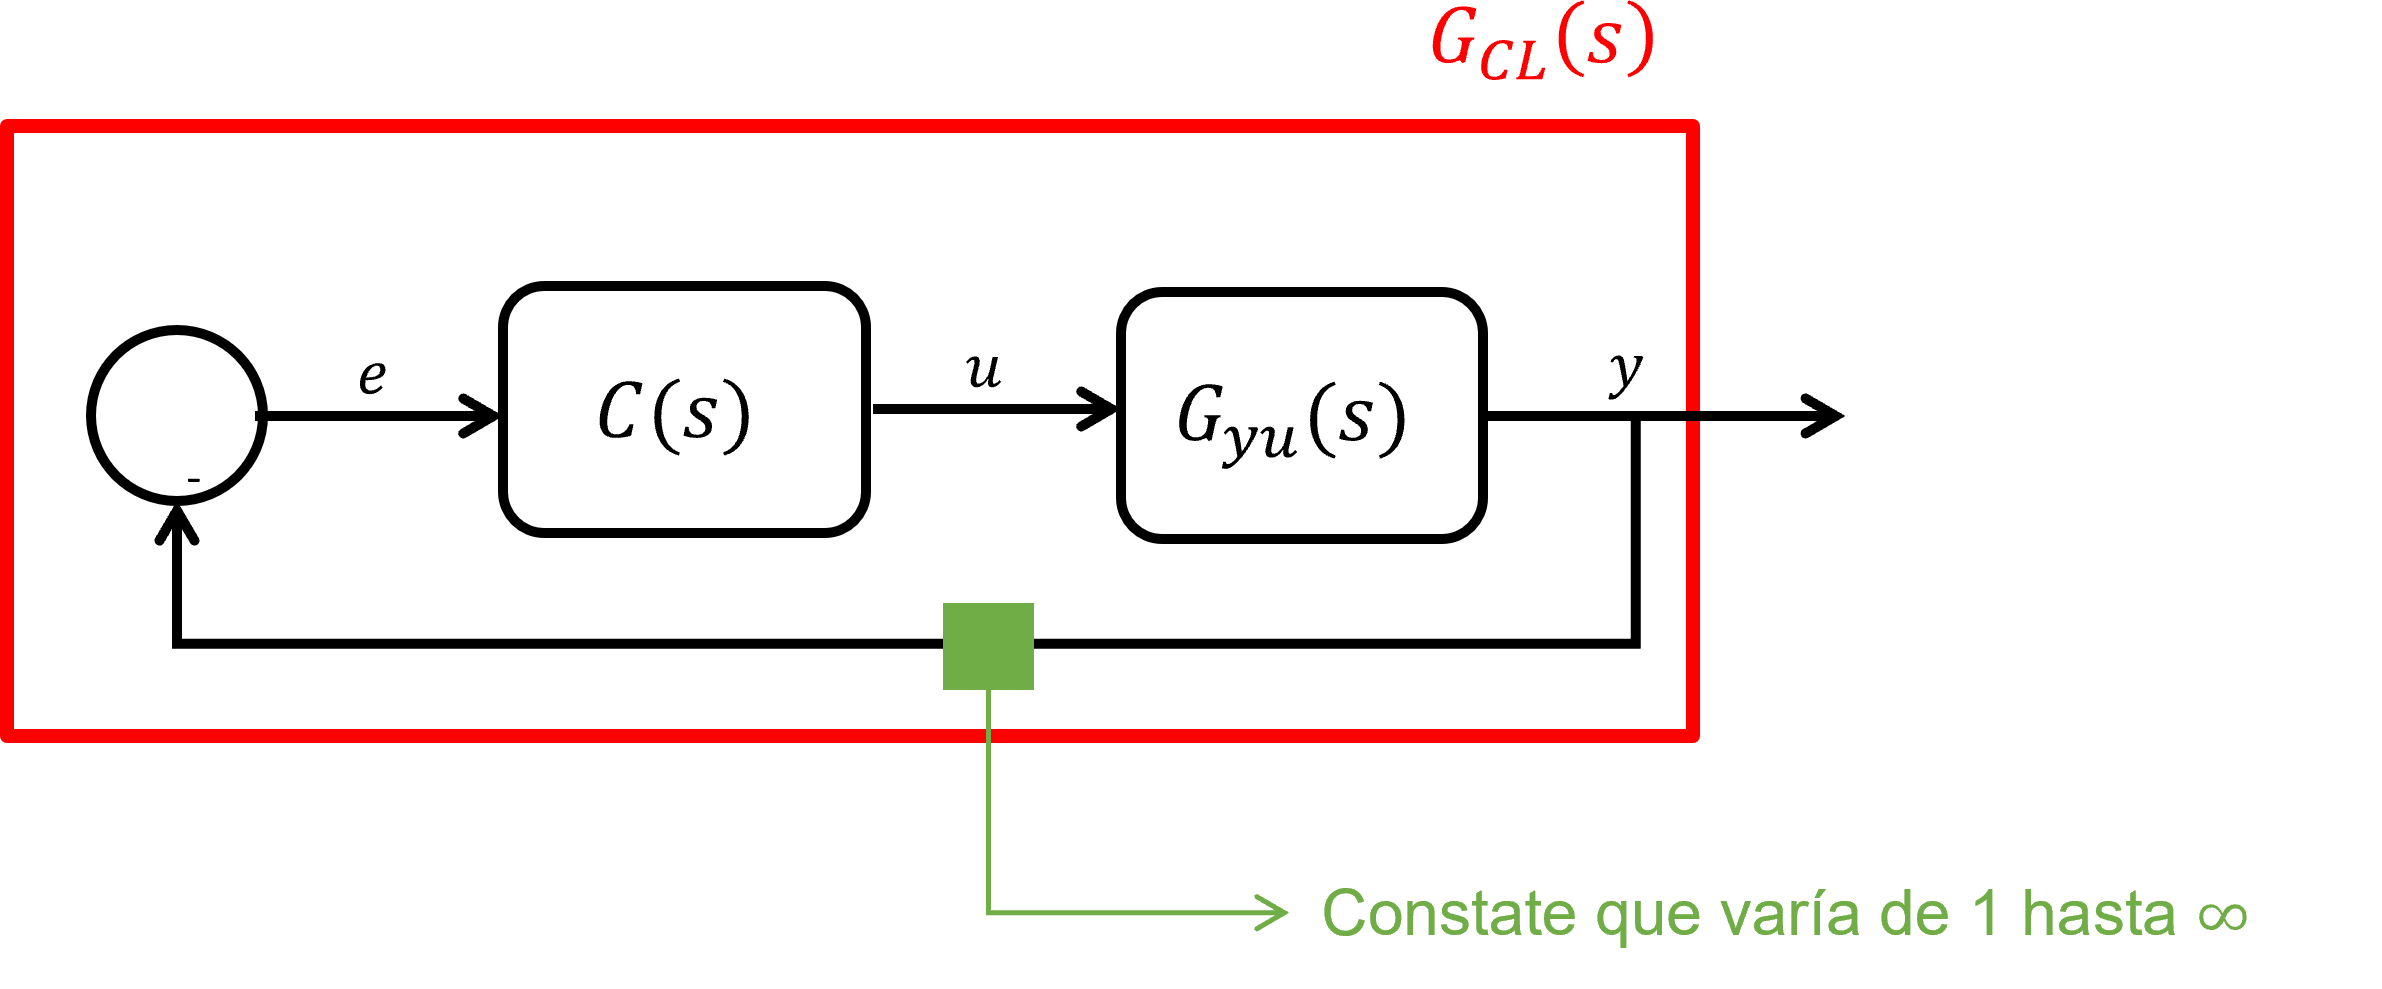
\includegraphics[scale=0.7]{Figuras/GCL.png}
\end{figure}

\begin{align*}
    G_{CL}(s)&=\frac{G(s)C(s)}{1+G(s)C(s)}\\
    G_{CL}(s)&=\frac{G(s)K_p\bigg(1+T_I/s+T_Ds\bigg)}{1+G(s)K_p\bigg(1+T_I/s+T_Ds\bigg)}
\end{align*}

\underline{Resumen control PID}: 
\begin{figure}[H]
\centering
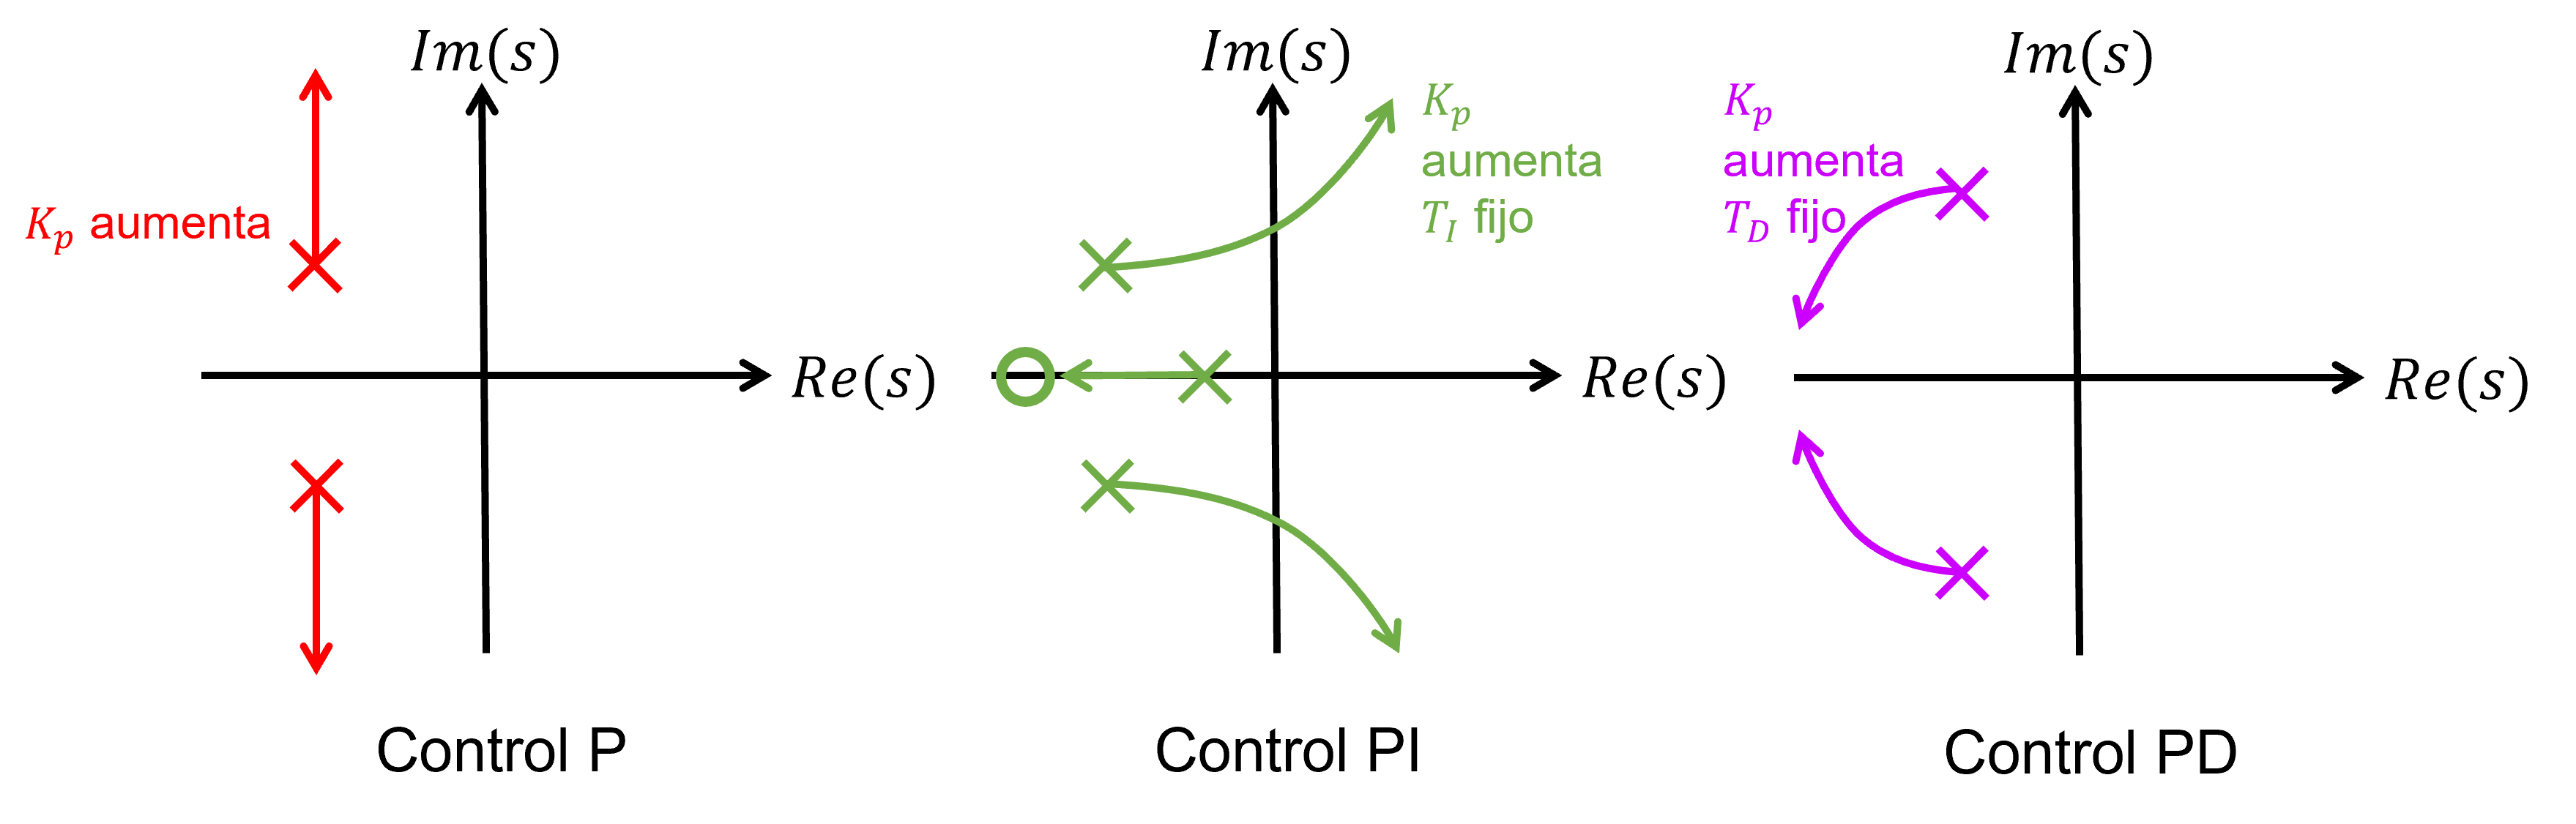
\includegraphics[scale=0.65]{Figuras/controlPID.png}
\end{figure}

\section{Control Moderno}
Representación espacio estado, sistema LTI.\\
\par Sea: 
\begin{align*}
    {x}&=[x_1,x_2,...,x_N]^\top\\
    {u}&=[u_1,u_2,...,u_p]^\top\\
    {y}&=[y_1,y_2,...,y_r]^\top
\end{align*}
\begin{itemize}
    \item[(1)] Ecuación de estado:
    $${\dot{x}}={A}{x}+{B}{u} $$
    \item[(2)] Ecuación de respuesta:
    $${y}={C}{x}+{D}{u} $$
\end{itemize}

\underline{Paréntesis}:
Aplicando la Transformada de Laplace a las ecuaciones de estado y respuesta de la representación espacio-estado:
\begin{align*}
    {\dot{x}}={A}{x}+{B}{u}\xrightarrow[]{\mathcal{L}}s{X}(s)={A}{X}(s)+{B}{U}(s)\\
    \Longrightarrow {X}(s)=(s{I}-{A})^{-1}{B}{U}(s)\\
    G_{xu}(s)=(s{I}-{A})^{-1}{B}
\end{align*}
\begin{align*}
    {y}={C}{x}+{D}{u}\xrightarrow[]{\mathcal{L}}s{Y}(s)={C}{X}(s)+{D}{U}(s)\\
    {Y}(s)=[{C}(s{I}-{A})^{-1}{B}+{D}]{U}(s)\\
    G_{yu}={C}(s{I}-{A})^{-1}{B}+{D}
\end{align*}


\section{Formas canónicas}
\subsection{Forma Canónica Controlable (CCF)}
Asumir que ${D}={0}$ (no hay componente ``feedthrough'' en la salida del sistema).
\begin{align*}
{A_c}=\left[
    \begin{array}{cccc|c}
     -a_1 & -a_2 & \dots & -a_{n-1} & -a_n\\ \hline
     1 & & & 0 & 0\\
       & 1 & & & \vdots\\
       & & \ddots & & \\
     0 & & & 1 & 0  
    \end{array}\right], \quad {A_c}\in \mathbb{R}^{n\times n}
\end{align*}
\begin{align*}
{B_c}=\left[
    \begin{array}{c}
     1 \\ \hline
     0\\
    \vdots\\
     0  
    \end{array}\right], \quad {B_c}\in \mathbb{R}^{n\times 1}
\end{align*}
\begin{align*}
{C_c}=\left[
    \begin{array}{cccc}
     b_1 & b_2 & \dots & b_n
    \end{array}\right], \quad {C_c}\in \mathbb{R}^{1\times n}
\end{align*}
\begin{align*}
    \text{Realización (SISO): }\quad 
    \left\{
    \begin{array}{l}
          {\dot{x}_c}={A_c}{x_c}+{B_c}u \\
          y={C_c}{x_c} \\
    \end{array} 
    \right. 
\end{align*}
Notar que:
\begin{align*}
    \dot{x}_1 &= -a_1x_1-a_2x_2 ... -a_nx_n+1\cdot u\\
    \dot{x}_2 &= x_1\\
    \dot{x}_3 &= x_2\\
    \vdots \\
    \dot{x}_n &= x_{n-1}
\end{align*}

Utilizando la transformada de Laplace, se obtiene la siguiente función de transferencia:
\begin{align*}
    G_{yu}(s)=\frac{b_1s^{n-1}+b_2s^{n-2}+...+b-n}{s^n+a_1s^{n-1}+a_2s^{n-2}+...+a_n} = \frac{\text{numerador orden n-1}}{\text{denominador orden n}} = \text{TF Propia}
\end{align*}

Se utiliza para diseñar controladores cuando todos los estados del sistema son conocidos.

\subsection{Forma Canónica Modal (MCF)}
Sea $G(s)=\frac{c_1}{s+p_1}+\frac{c_2}{s+p_2}+...+\frac{c_n}{s+p_n}$, $G(s)$ se escribe como una expansión de fracción parcial, y los polos $p_i$ son todos distintos:
\begin{align*}
{A_m}=\left[
    \begin{array}{cccc}
     -p_1& & & 0\\
     & -p_2 & & \\
     & & \ddots & \\
     0 & & & -p_n
    \end{array}\right], \quad {A_m}\in \mathbb{R}^{n\times n}
\end{align*}
\begin{align*}
{B_m}=\left[
    \begin{array}{c}
     1 \\ 
     1\\
    \vdots\\
     1  
    \end{array}\right], \quad {B_m}\in \mathbb{R}^{n\times 1}
\end{align*}
\begin{align*}
{C_m}=\left[
    \begin{array}{cccc}
     c_1 & c_2 & \dots & c_n
    \end{array}\right], \quad {C_m}\in \mathbb{R}^{1\times n}
\end{align*}

\begin{align*}
    \text{Realización (SISO): }\quad 
    \left\{
    \begin{array}{l}
          {\dot{x}_m}={A_m}{x_m}+{B_m}\cancelto{0}{u} 
    \end{array} 
    \right. 
\end{align*}

\begin{align*}
    \dot{x}_{m_1} &= \lambda_1x_{m_1}\\
    \dot{x}_{m_2} &= \lambda_2x_{m_1}\\
    \vdots \\
    \dot{x}_{m_n} &= \lambda_nx_{m_n}
\end{align*}

\begin{align*}
    \Longrightarrow{\dot{x}}={A}{x}
\end{align*}

\underline{Resolver}: ${A}{v}=\lambda {v}$ (Problema de valores propios de ${A}$).\\
\par ${T}$ es la matriz de transformación modal, ${T}=[{v_1},{v_2},...,{v_n}]$\\

\subsection{Forma Canónica Observable (OCF)}
Dado $G(s)=\frac{n(s)}{d(s)}$, con $a_i$, $b_i$ conocidos.

\begin{align*}
{A_o}=\left[
    \begin{array}{c|cccc}
     -a_{n-1} & 1 & & & 0 \\ 
     -a_{n-2} & & 1 & & \\
     \vdots   & & & \ddots & \\
     -a_1     & 0 & & & 1 \\ \hline
     -a_0     & 0 & 0 & \dots & 0   
    \end{array}\right], \quad {A_o}\in \mathbb{R}^{n\times n}
\end{align*}
\begin{align*}
{B_o}=\left[
    \begin{array}{c}
     b_{n-1} \\
     b_{n-2}\\
    \vdots\\
     b_1 \\ \hline
     b_0
    \end{array}\right], \quad {B_o}\in \mathbb{R}^{n\times 1}
\end{align*}
\begin{align*}
{C_o}=\left[
    \begin{array}{c|ccc}
     1 & 0 & \dots & 0
    \end{array}\right], \quad {C}_o\in \mathbb{R}^{1\times n}
\end{align*}

Se utiliza para diseñar ``observadores''.


\section{Control lazo cerrado utilizando estados (State Feedback Control)}

\begin{figure}[H]
\centering
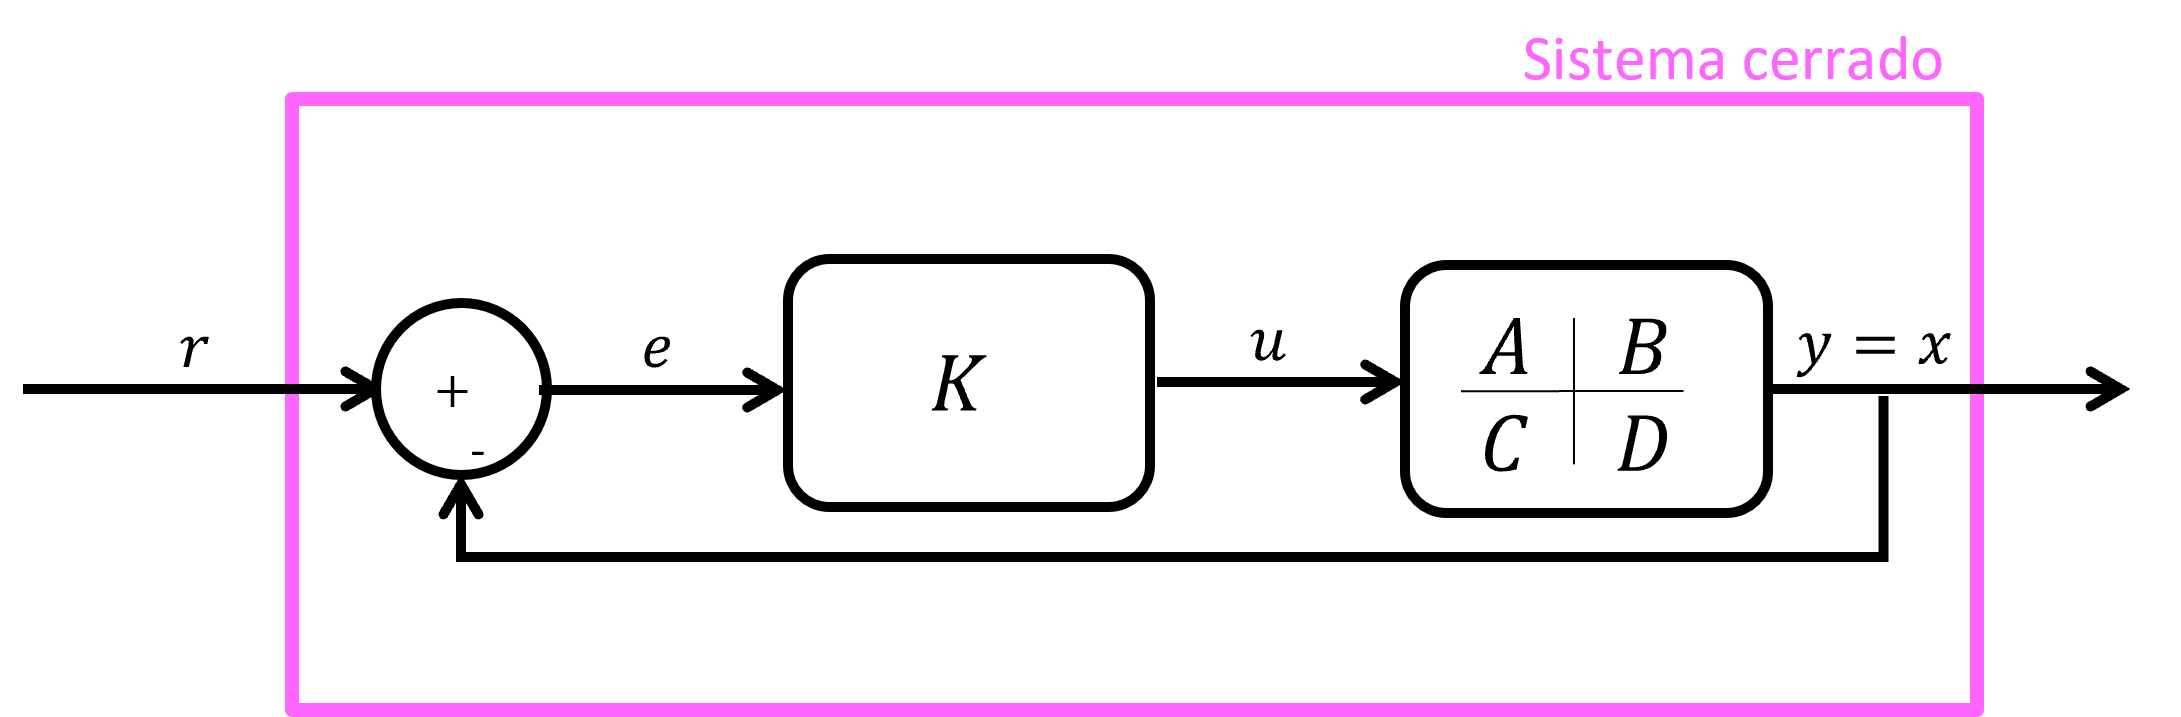
\includegraphics[scale=0.7]{Figuras/State_feedback.png}
\end{figure}
\underline{Objetivo}: Diseñar $K$ tal que $e=r-x\to 0$ para un tiempo $t_f$.\\
\par \underline{Definición}: El sistema de control ``full state feedback'' tiene relación con el hecho que el controlador cuenta con acceso a todos los estados del sistema.\\

\par Veamos la ecuación de estado del sistema:
\begin{align*}
    \dot{x}=Ax+Bu
\end{align*}
La señal de control:
\begin{align*}
    u=Ke
\end{align*}
La señal de error:
\begin{align*}
    e=r-x
\end{align*}

Luego:

\begin{align*}
    \dot{x} &= Ax+BK(r-x)\\
    \dot{x} &= (A-BK)x+BKr\\
\end{align*}

\begin{itemize}
    \item $A_{CL}=A-BK$: matriz de estado del sistema cerrado.
    \item $B_{CL}=BK$
\end{itemize}

\begin{align*}
    \dot{x}=A_{CL}x+B_{CL}r
\end{align*}

Para que el sistema cerrado sea \textcolor{red}{ESTABLE}, los valores propios de $A_{CL}$ deben tener partes reales estrictamente negativas:

\begin{align*}
    \Re(\text{eig}(A_{CL}))<0
\end{align*}

\par Analicemos el diseño de un controlador utilizando una representación CCF:

\begin{align*}
{A}=\left[
    \begin{array}{cccc|c}
     -a_1 & -a_2 & \dots & -a_{n-1} & -a_n\\ \hline
     1 & & & 0 & 0\\
       & 1 & & & \vdots\\
       & & \ddots & & \\
     0 & & & 1 & 0  
    \end{array}\right]_{n\times n}
\end{align*}
\begin{align*}
{B}=\left[
    \begin{array}{c}
     1 \\ \hline
     0\\
    \vdots\\
     0  
    \end{array}\right]_{n\times 1}
\end{align*}
\begin{align*}
{K}=\left[
    \begin{array}{ccccc}
     k_{n-1} & k_{n-2} & \dots & k_1 & k_0
    \end{array}\right]_{1\times n}
\end{align*}

Calculemos $BK$:
\begin{align*}
{BK}=\left[
    \begin{array}{cccc|c}
     k_{n-1} & k_{n-2} & \dots & k_1 & k_0\\ \hline
      & & & & 0\\
      & & {0}_{(n-1)\times(n-1)} & & \vdots\\
      & & & & 0  
    \end{array}\right]_{n\times n}
\end{align*}

Ahora, calculemos $A_{CL}=A-BK$
\begin{align*}
{BK}=\left[
    \begin{array}{cccc|c}
     -(a_{n-1}+k_{n-1}) & -(a_{n-2}+k_{n-2}) & \dots & -(a_1+k_1) & -(a_0+k_0)\\ \hline
      & & & & 0\\
      & & {I}_{(n-1)\times(n-1)} & & \vdots\\
      & & & & 0  
    \end{array}\right]_{n\times n}
\end{align*}

Queremos encontrar los valores propios de $A_{CL}$. Escribamos la ecuación característica de $A_{CL}$
\begin{align*}
    \det({A_{CL}}-\lambda {I})=0
\end{align*}

\begin{align*}
{BK}=\left[
    \begin{array}{cccc|c}
     -(\lambda+a_{n-1}+k_{n-1}) & -(a_{n-2}+k_{n-2}) & \dots & -(a_1+k_1) & -(a_0+k_0)\\ \hline
      1 & -\lambda & & & 0\\
      & 1 & -\lambda & & \vdots\\
      & & \ddots & \ddots & 0\\
      & & & 1 & -\lambda\\
    \end{array}\right]=0
\end{align*}

La ecuación característica resulta ser:
\begin{align*}
    \lambda^n+(a_{n-1}+k_{n-1})\lambda^{n-1}+(a_{n-2}+k_{n-2})\lambda^{n-2}+...+(a_{1}+k_{1})\lambda+(a_{0}+k_{0})=0
\end{align*}
Si queremos ubicar los polos en una posición particular, o sea, queremos fijar los polos de la siguiente manera:
$$ \lambda=\{p_1,p_2,p_3,..,p_n \}$$

Podemos reescribir la ecuación característica de la siguiente forma:
$$(\lambda-p_1)(\lambda-p_2)(\lambda-p_3)...(\lambda-p_n)=0 $$

Desarrollando el polinomio:
$$\Longrightarrow \lambda^n+\alpha_{n-1}\lambda^{n-1}+...+\alpha_1\lambda+\alpha_0=0 $$
Entonces, el controlador $K$ se define como:
\begin{align*}
    \alpha_{n-1} = a_{n-1}+k_{n-1} &\Longrightarrow k_{n-1} = \alpha_{n-1}-a_{n-1}\\
    \alpha_{n-2} = a_{n-2}+k_{n-2} &\Longrightarrow k_{n-2} = \alpha_{n-2}-a_{n-2}\\
    \vdots \\
    \alpha_0 = a_0+k_0 &\Longrightarrow k_0 = \alpha_0-a_0\\
\end{align*}

Donde $\alpha_i$ se obtiene de la posición deseada de los polos. \\

\par Entonces, si el sistema es CCF, podemos diseñar $K$ al elegir la posición de los polos de manera apropiada $\Longrightarrow$ \textbf{POLE PLACEMENT}\\

\par \underline{Nota}: Si el sistema no es CCF, entonces se puede transformar a CCF utilizando matriz de transformación ${T}$, provisto que el sistema sea controlable.\\

\par Sea la realización:

\begin{align*}
    {x}=Ax+Bu \xrightarrow[]{x=Tz} \dot{z}=A_cz+B_cu
\end{align*}
Sea $T \in \mathbb{R}^{n\times n}$, tal que $T^{-1}$ existe
\begin{align*}
    \Longrightarrow x&=Tz\\
    \Longrightarrow \dot{x}&=T\dot{z}
\end{align*}
Reemplazando:
\begin{align*}
    T\dot{z} &= ATz+Bu\\
    \Longrightarrow \dot{z}&=T^{-1}ATz+T^{-1}Bu\\
    \dot{z} &= A_cz+B_cu
\end{align*}

``Pole placement'', pasos a seguir:
\begin{enumerate}
    \item Buscar $T$ y transformar a CCF ($A_c$ y $B_c$).
    \item Encontrar $K_c$ , en base a la ubicación de polos deseados.
    \item Volver al sistema original (asuma $r=0$)
\end{enumerate}
\begin{align*}
    \Longrightarrow \dot{z} &= (A_c-B_cK_c)z\\
    \Longrightarrow T\dot{z} &= TA_cz+TB_cz\\
    \Longrightarrow \dot{x} &= TT^{-1}ATz-TT^{-1}BK_cz\\
    \Longrightarrow \dot{x} &= Ax-BK_cT^{-1}x\\
    \Longrightarrow \dot{x} &= (A-BK)x
\end{align*}
donde  $K=K_cT^{-1}$, controlador para el sistema original.

\section{Observadores}
\underline{Motivación}: \\

Considere el siguiente ejemplo de sistema dinámico:
\begin{align*}
    \dot{x} &= f(x,u)\\
    y &= g(x,u)
\end{align*}

\begin{figure}[H]
\centering
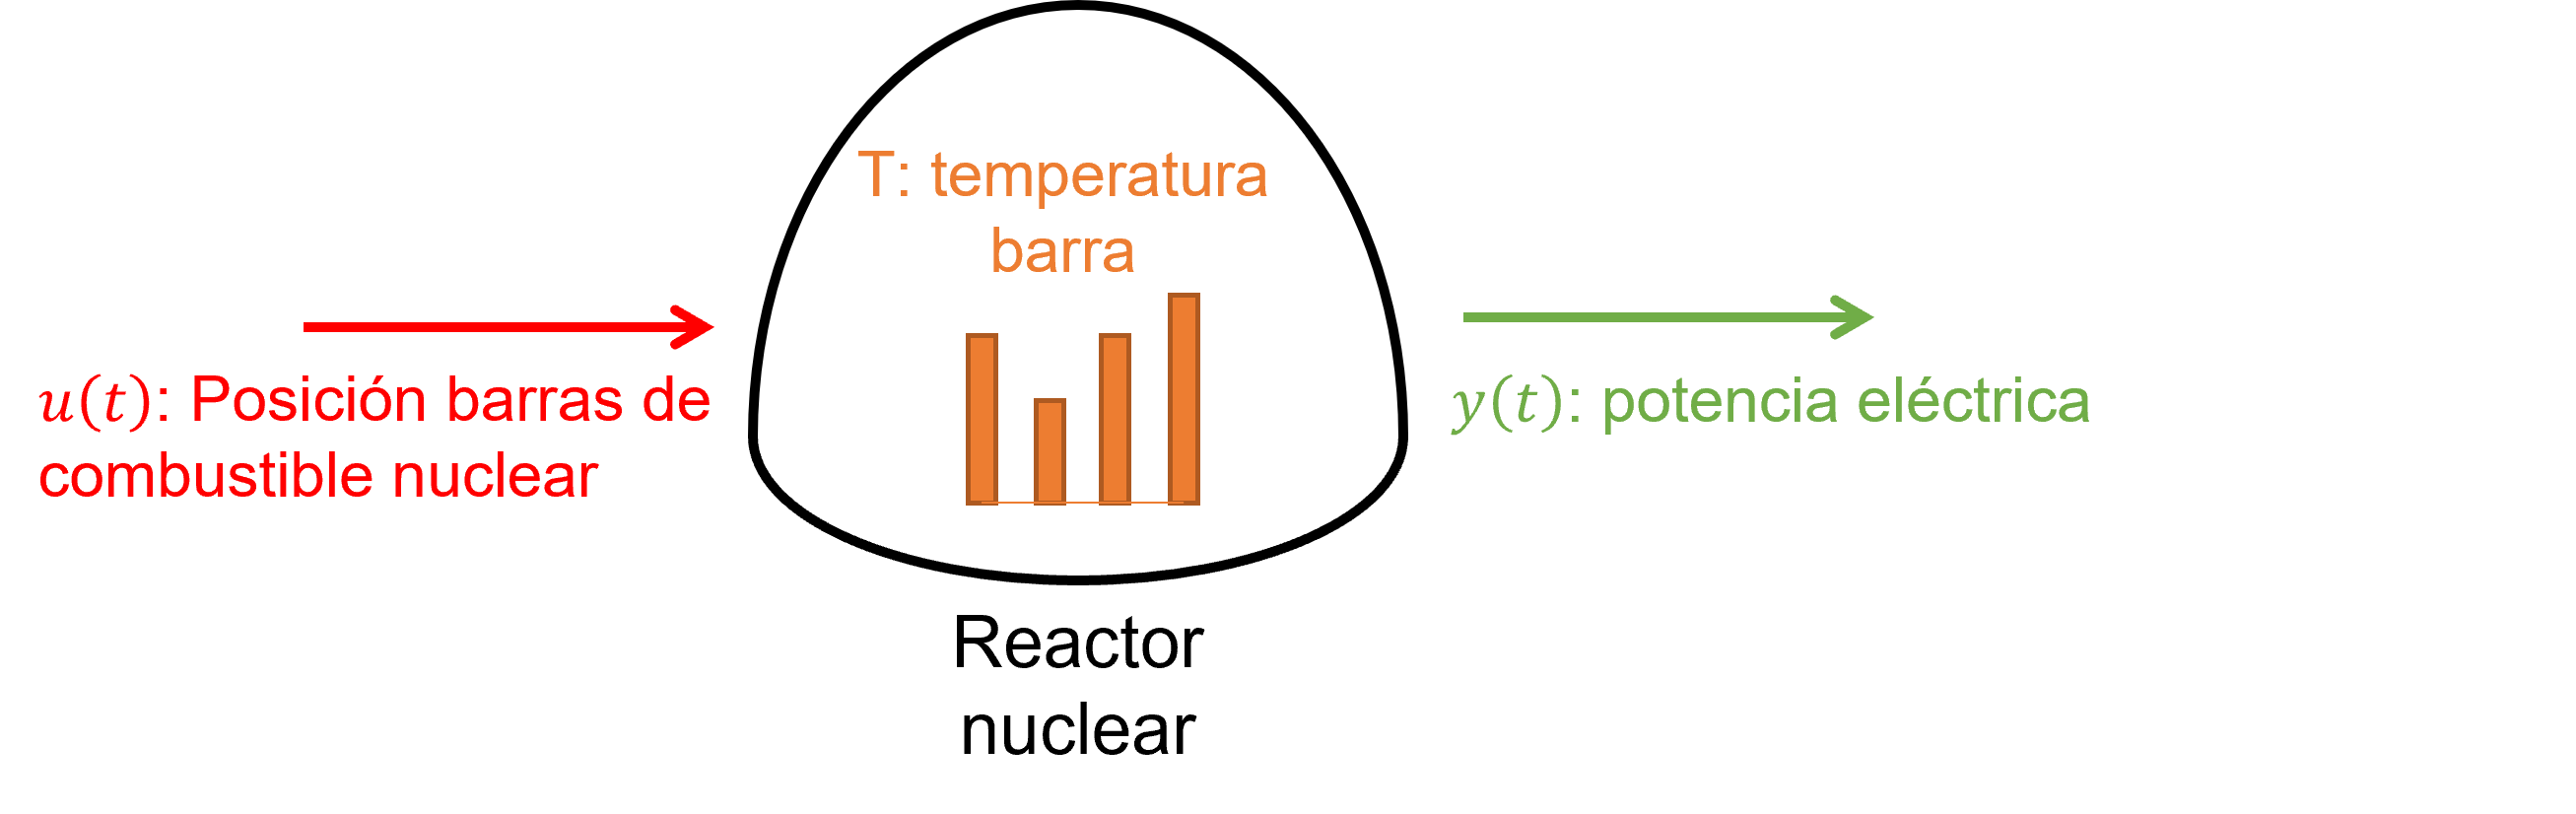
\includegraphics[scale=0.7]{Figuras/nuclear.png}
\end{figure}
¿Es posible determinar los estados internos del sistema $x(t)$ (temperatura de las barras), utilizando solo las señales de entrada y salida $\{u(t), y(t)\}$? La respuesta es sí, pero con la condición de que el sistema sea \textbf{observable}.\\

El objetivo de lo que se desarrollará a continuación es \emph{diseñar} un \emph{observador/estimador} para poder estimar los estados internos $x(t)$ de un sistema, de tal forma que dependa únicamente de las señales de entrada y salida del sistema:

\begin{align*}
    \hat{x}(t) = f(u(t), y(t))
\end{align*}

\begin{figure}[H]
\centering
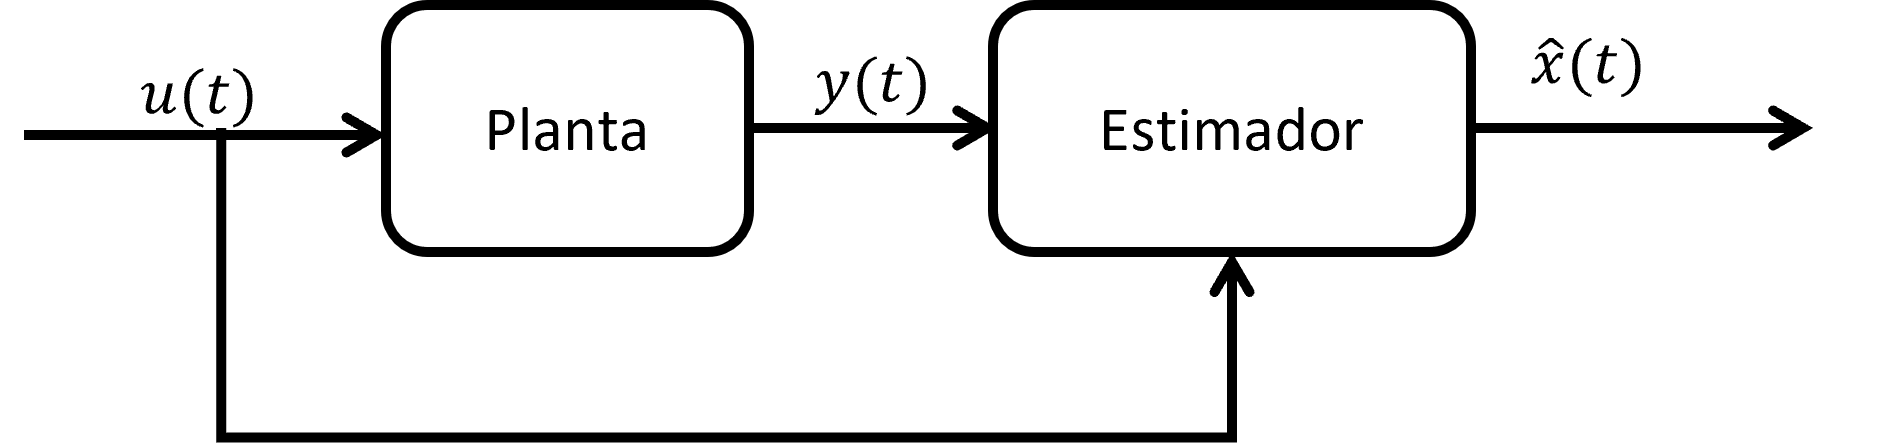
\includegraphics[scale=0.7]{Figuras/observador2.png}
\end{figure}

\underline{Notación}:
\begin{itemize}
    \item $x(t)$: estados del sistema
    \item $\hat{x}(t)$: estados estimados
    \item $\tilde{x}(t)=x(t)-\hat{x}(t)$: error de estimación
\end{itemize}

La dinámica del sistema de los \emph{estados estimados} $\hat{x}$ es la misma que la del sistema planta:

\begin{align*}
    &\dot{\hat{x}} = A\hat{x}+Bu \\
    &\hat{x}(0) = \hat{x}_0    
\end{align*}

Luego, se puede deducir la dinámica del \emph{error de estimación} $\tilde{x}$:

\begin{align*}
    \dot{\tilde{x}} &= \frac{d}{dt}(x-\hat{x})=\dot{x}-\dot{\hat{x}}\\
    &= (Ax+Bu)-(A\hat{x}+Bu)=A(x-\hat{x}) \\
    \Longrightarrow \dot{\tilde{x}} &= A\tilde{x} 
\end{align*}

La estrategia para diseñar el observador es la siguiente: Si los estados decaen a cero, entonces se diseña un estimador tal que el error de la estimación decae con la misma tasa que el sistema.

\begin{figure}[H]
\centering
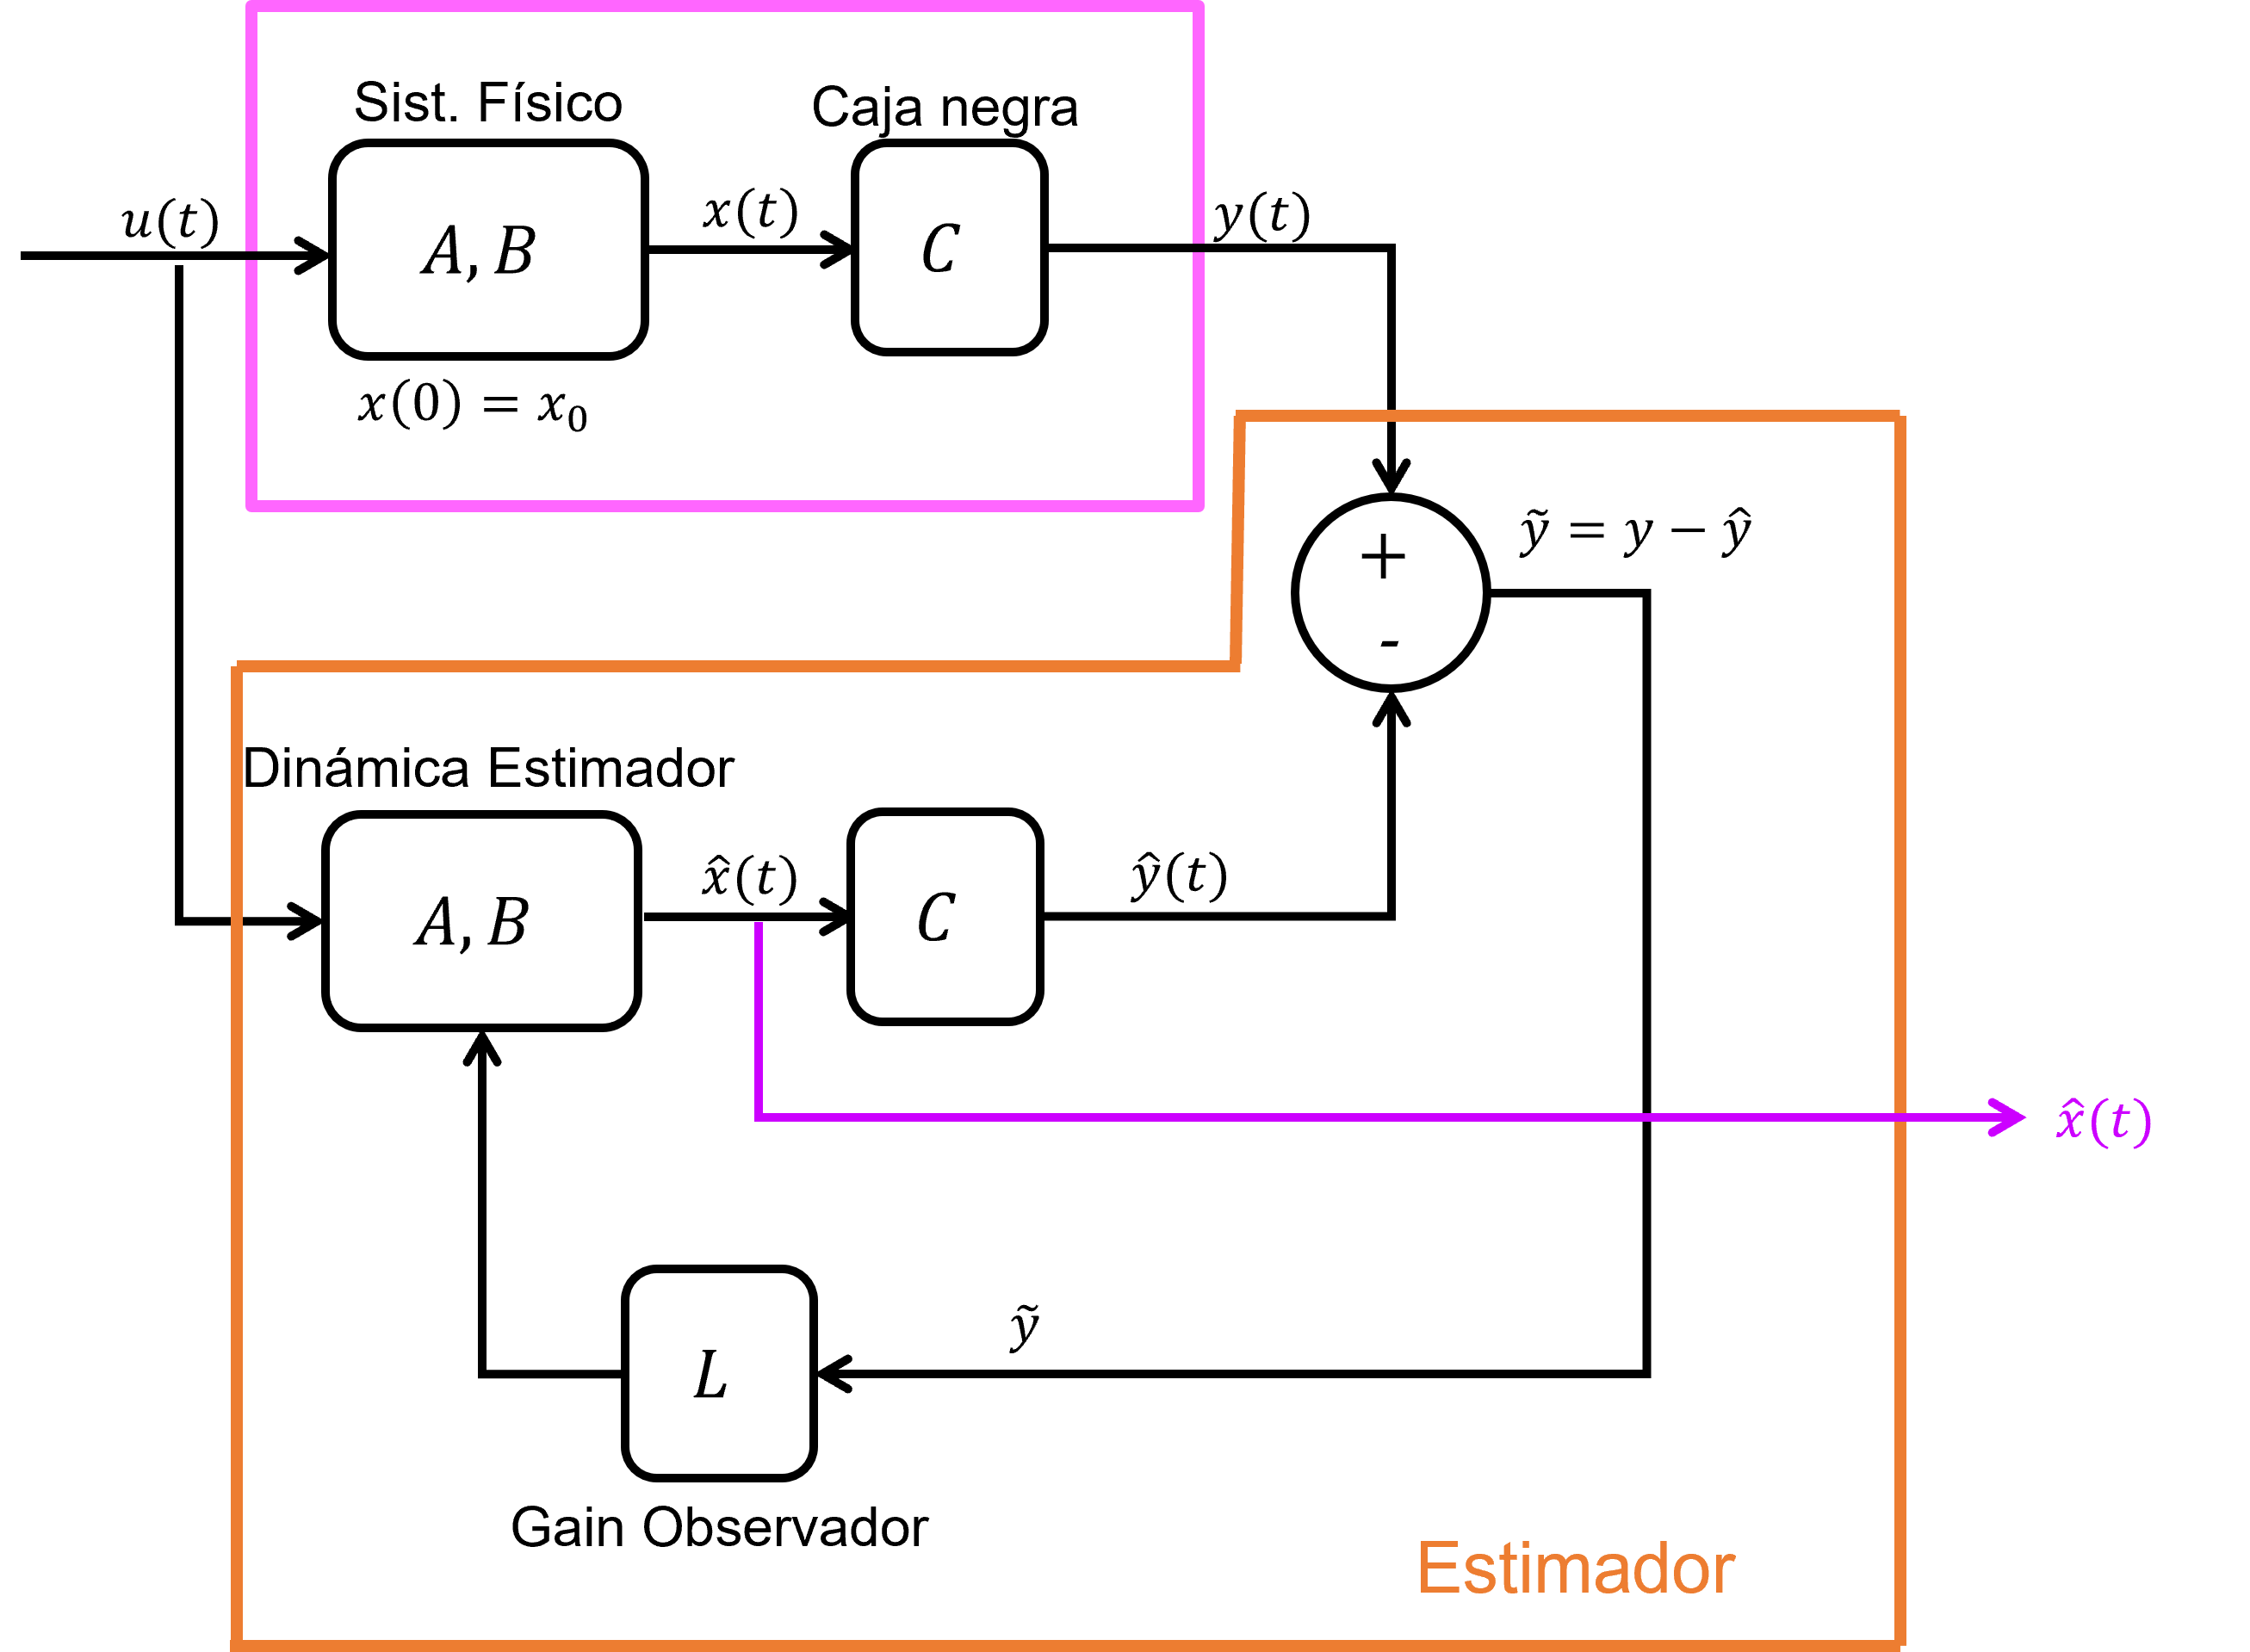
\includegraphics[scale=0.8]{Figuras/observador.png}
\end{figure}

\section{Diseño de Observador de Estados}
De la figura anterior, notar que para estimar los estados del sistema, se requiere de una ganancia $L$. Lo que se va a realizar a continuación es diseñar esta matriz $L$. \\

La representación espacio-estado de los estados estimados $\hat{x}(t)$ incluye la señal del error de estimación $\tilde{x}$ y su ganancia $L$.

\begin{align*}
    \dot{\hat{x}}(t) = A\hat{x}(t)+Bu(t)+L\tilde{y}(t)
\end{align*}
donde:
\begin{align*}
    L=\left[
    \begin{array}{c}
     l_1 \\ l_2\\ \vdots\\ l_n 
    \end{array}\right], \quad L \in \mathbb{R}^{n\times r}, \quad x,y \in \mathbb{R}^n 
\end{align*}

La ecuación de estado del error de estimación queda de la siguiente forma:
\begin{align*}
    \dot{\tilde{x}}=\dot{x}-\dot{\hat{x}} &= (Ax+Bu)-(A\hat{x}+Bu+L\tilde{y})\\
    &= A\tilde{x}-L(y-\hat{y})\\
    &= A\tilde{x}-L(Cx-C\hat{x})\\
    &= A\tilde{x}-LC\tilde{x}\\
    \dot{\tilde{x}} &= (A-LC)\tilde{x}
\end{align*}

Por lo tanto, para diseñar $L$, $(A-LC)$ debe cumplir con estabilidad. Para lograr esta estabilidad, se ubicarán apropiadamente los polos de forma que se encuentren al lado izquierdo del plano complejo. A esta estrategia se le conoce como \textbf{Pole Placement}. \\

\underline{Caso particular}: 

Considere el siguiente sistema con $x\in\mathbb{R}^n$, $u\in\mathbb{R}$, $y\in\mathbb{R}$: 

\begin{align*}
    G(s) = \frac{b_0}{s^n+a_{n-1}s^{n-1}+...+a_1s+a_0}
\end{align*}

Su Forma Canónica Observable es: 

\begin{align*}
{A_o}=\left[
    \begin{array}{c|cccc}
     -a_{n-1} & 1 & & & 0 \\ 
     -a_{n-2} & & 1 & & \\
     \vdots   & & & \ddots & \\
     -a_1     & 0 & & & 1 \\ \hline
     -a_0     & 0 & 0 & \dots & 0   
    \end{array}\right], \quad {A_o}\in \mathbb{R}^{n\times n}
\end{align*}
\begin{align*}
{B_o}=\left[
    \begin{array}{c}
     b_{n-1} \\
     b_{n-2}\\
    \vdots\\
     b_1 \\ \hline
     b_0
    \end{array}\right], \quad {B_o}\in \mathbb{R}^{n\times 1}
\end{align*}
\begin{align*}
{C_o}=\left[
    \begin{array}{c|ccc}
     1 & 0 & \dots & 0
    \end{array}\right], \quad {C}_o\in \mathbb{R}^{1\times n}
\end{align*}

Como en este caso particular, $y\in\mathbb{R}$, entonces $L$ es matriz $n \times 1$:
\begin{align*}
    L=\left[
    \begin{array}{c}
     l_{n-1} \\ l_{n-2}\\ \vdots\\ l_0 
    \end{array}\right] 
\end{align*}
%\underline{Objetivo}: Determinar los $l_i$, $i\in[0,n-1]$

Por lo tanto, se puede obtener $A_0 - LC_0$ de la siguiente forma:
\begin{align*}
    LC_o&=\left[
    \begin{array}{c}
     l_{n-1} \\ l_{n-2}\\ \vdots\\ l_0 
    \end{array}\right] \left[
    \begin{array}{c c c c}
     1 & 0 & ... & 0
    \end{array}\right] =\left[
    \begin{array}{c|c}
     l_{n-1} & \\ \vdots & {0} \\ l_0 & 
    \end{array}\right] \\
    A_o-LC_o &= \left[ \begin{array}{c|c c c}
     -a_{n-1}-l_{n-1} & & & \\  -a_{n-2}-l_{n-2} & & & \\ \vdots & & {I} & \\-a_1-l_1 & & & \\ \hline \\ -a_0-l_0 & 0 & ... & 0
    \end{array}\right] 
\end{align*}
y su ecuación característica es: 
\begin{align*}
    &\phantom{\Longrightarrow} \Delta(A_o-LC_o) = 0 \\
    &\Longrightarrow s^n+(a_{n-1}+l_{n-1})s^{n-1}+...+(a_1+l_1)s+(a_0+l_0) = 0
\end{align*}

Cada coeficiente $(a_i+l_i)$, son los coeficientes $\lambda_i$ del polinomio característico asociado a la ubicación de polos deseada $p_i$:

\begin{align*}
    \prod_{i=0}^{n-1}(s-p_i)=s^n+\lambda_{n-1}s^{n-1}+...+\lambda_1s+\lambda_0=0
\end{align*}

Para finalmente obtener los términos $l_i$ de la matriz $L$, se deben definir los polos deseados, expandir el polinomio y luego igualar ambos términos para todo $i \in [0,n-1]$.

\begin{align*}
    &\phantom{\longrightarrow} a_i + l_i = \lambda_i \\
    &\longrightarrow l_i = a_i-\lambda_i
\end{align*}

\underline{Nota}: En MATLAB, el diseño por ubicación de polos se puede realizar utilizando el comando \texttt{place()}. \\

\underline{Nota}: Si el sistema no está escrito en OCF (forma canónica observable), es recomendable transformarlo a OCF con una transformación de similitud utilizando la matriz $T$. Recordar que esta matriz $T$ existe ssi el sistema es observable.


\section{Principio de Separación}
Considere el siguiente sistema LTI cerrado:
\begin{figure}[H]
\centering
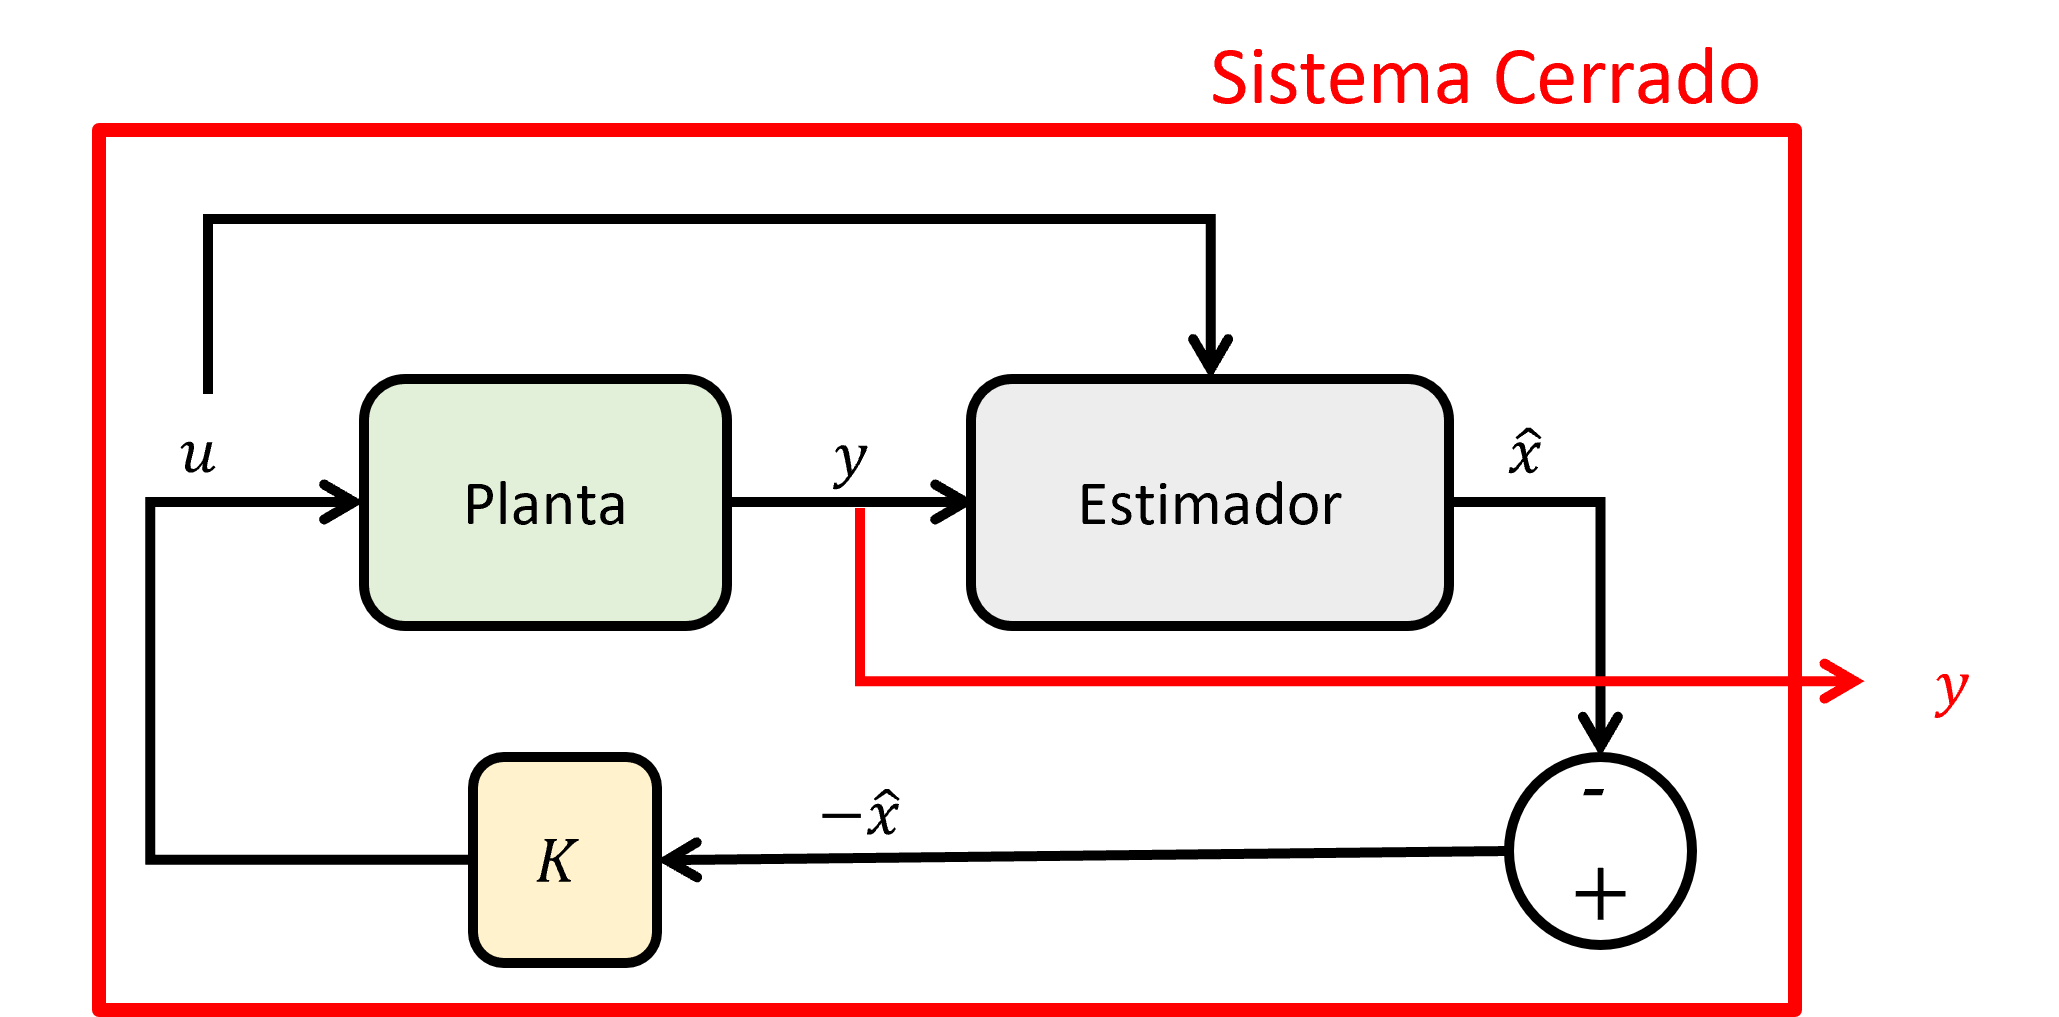
\includegraphics[scale=0.7]{Figuras/ppio_separacion.png}
\end{figure}


Planta:
\begin{subequations}
    \begin{align}
        \dot{x} &= Ax+Bu\\
        y &= Cx
    \end{align}
\end{subequations}

Controlador:
\begin{subequations}
    \begin{align}
        u = -K\hat{x}
    \end{align}
\end{subequations} 

Estimador y error de estimación:
\begin{subequations}
    \begin{align}
        \dot{\hat{x}}&= A\hat{x}+Bu+L\tilde{y}\\
        \hat{y} &= C\hat{x}\\
        \tilde{x} &= x-\hat{x}\\
        \tilde{y} &= y-\hat{y}
    \end{align}
\end{subequations}

Utilizando las ecuaciones de cada subsistema, vamos a obtener una expresión para el sistema cerrado: \\

Reemplazando (2.3c) en (2.2a):
\begin{align*}
    u&=-K(x-\tilde{x})\\
\end{align*}

Reemplazando lo anterior en (2.1a):
\begin{align*}
    \dot{x} &= Ax + B(-K(x - \tilde{x}))\\
    \Longrightarrow \dot{x} &= Ax - BK(x-\tilde{x}) \\
    \Longrightarrow \dot{x} &= (A-BK)x+BK\tilde{x}
\end{align*}

Restando (2.1a) menos (2.3a) para obtener la dinámica del error de estimación
\begin{align*}
    \Longrightarrow \dot{\tilde{x}} &= (Ax+Bu)-(A\hat{x}+Bu+L\tilde{y})\\
    \Longrightarrow \dot{\tilde{x}} &= A\tilde{x}-LC \tilde{x}\\
    \Longrightarrow \dot{\tilde{x}} &= (A-LC)\tilde{x}
\end{align*}

Luego, definiendo los estados del sistema cerrado como $z=\left[
    \begin{array}{c}
     x \\ \tilde{x} 
    \end{array}\right]$

La ecuación de estado del sistema cerrado queda de la siguiente forma:
\begin{align*}
    \dot{z}=\left[
    \begin{array}{c}
     \dot{x} \\ \dot{\tilde{x}} 
    \end{array}\right] = \left[
    \begin{array}{cc}
     A-BK & BK \\ 0 & A-LC 
    \end{array}\right]\left[
    \begin{array}{c}
     x \\ \tilde{x} 
    \end{array}\right]
\end{align*}

Para simplificar notación, la matriz de estado del sistema cerrado se denotará como $A_{CL}$
\begin{align*}
    A_{CL} &= \left[
    \begin{array}{cc}
     A-BK & BK \\ 0 & A-LC 
    \end{array}\right]\\
    \Longrightarrow \dot{z}&=A_{CL}z
\end{align*}

Finalmente, los polos de $A_{CL}$ se obtienen al resolver la ecuación característica:
\begin{align*}
    \text{det}(sI-A_{CL})&=0\\
    \Longrightarrow \text{det}(sI-(A-BK))\cdot\text{det}(sI-(A-LC)) &=0
\end{align*}

\begin{itemize}
    \item $\text{det}(sI-(A-BK))$: polos del subsistema planta + controlador
    \item $\text{det}(sI-(A-LC))$: polos del subsistema planta + observador 
\end{itemize}

Este resultado se conoce como \textbf{Principio de Separación}.\\

Con este principio, se puede diseñar $K$ y $L$ por separado, luego agrupar y construir el sistema de control cerrado.

